\documentclass[../document.tex]{subfiles}

\begin{document}
    \section{Реализация методов и тестирование}
        \subsection{Описание проекта}
            \par \par Разрабатываемая в данной работе программа является усовершенствованием программы, написанной в рамках выпускной квалификационной работы бакалавра \cite{bachelor}. Исходный код программы расположен в открытом доступе по адресу: \url{https://github.com/GoldFeniks/Ample}. В рамках данной работы было сделано 70 коммитов, добавлено 12500 и удалено 7000 строк кода на языке программирования C++.  
            \subsubsection{Средства реализации}
                \par В качестве основного языка программирования для реализации проекта был выбран язык C++17 \cite{c++}, ввиду следующих соображений:
                \begin{enumerate}
                    \item C++ является современным кроссплатформенным развивающимся языком программирования;
                    \item С++ позволяет проводить эффективное управление памятью;
                    \item C++ поддерживает параллельные вычислению;
                    \item Программы, написанные на языке C++, зачастую работают быстрее аналогичных программ, написанных на других языках программирования;
                    \item Стандартная библиотека C++ имеет широкий функционал;
                    \item Для C++ существует большой набор библиотек, упрощающих разработку;
                    \item Пакет CAMBALA \cite{cambala} написан на C++, что упрощает его интеграцию.
                \end{enumerate}
            \subsubsection{Требования к аппаратному обеспечению}
                \begin{itemize}
                    \item Процессор Intel Core i7 2.5 ГГц;
                    \item 8 Гб оперативной памяти.
                \end{itemize}
            \subsubsection{Требования к программному обеспечению}
                \begin{itemize}
                    \item ОС Linux 5.12.2 и выше, и другие ОС, для которых существует компилятор языка C++17 \cite{c++};
                    \item Библиотека Boost \cite{boost} версии 1.69 и выше;
                    \item Библиотека nlohmann/json \cite{nlohmann} версии 3.9.1 и выше;
                    \item Библиотека FFTW \cite{fftw3,fftw05} версии 3.3.9 и выше.
                \end{itemize}
            \subsubsection{Требования к пользователю}
                \begin{itemize}
                    \item Умение пользоваться командной строкой;
                    \item Понимание работы с текстовыми и бинарными файлами;
                    \item Знание формата JSON \cite{json};
                    \item Понимание предметной области.
                \end{itemize}
            \subsubsection{Используемые модули}
                \begin{itemize}
                    \item CAMBALA \cite{cambala} -- используется для вычисления модовых функций и соответствующих им горизонтальных волновых чисел (см. \ref{sec::sound_modes});
                    \item DORK \cite{dork} -- реализация обобщённого метода Рунге-Кутты и плотной выдачи \cite{dense}, используется при вычислении координат распространения лучей, соответствующих вертикальным модам (см. \ref{sec::horizontal_rays});
                    \item delaunay \cite{delaunay} -- реализация S-hull алгоритма триангуляции \cite{shull}, используется для интерполяции данных гидрологии на облаке точек;
                    \item zip \cite{zip} -- C++ реализация функции zip, аналогично языку программирования Python.
                    \item Eigen \cite{eigenweb} -- библиотека, содержащая различные инструменты для линейной алгебры: векторы, матрицы, численные методы и прочие алгоритмы.
                \end{itemize}
            \subsubsection{Структура проекта}
                \begin{itemize}
                    \item\code{boundary_conditions} -- содержит реализацию \acrshort{pml} граничных условий с возможностью использования произвольной функции $\beta\pa{y}$;
                    \item\code{coefficients} -- функции для вычисления аппроксимаций Паде произвольного порядка;
                    \item\code{config} -- класс, предоставляющий интерфейс взаимодействия с конфигурационным файлом (см. конфигурационный файл);
                    \item\code{initial_conditions} -- класс для вычисления различных начальных условий: начальное условие Гаусса \eqref{eq::gauss}, начальное условие Грина \eqref{eq::greene}, обобщённый источник Гаусса\parencite{jensen} \cite{jensen}, лучевые начальные условия (см. \ref{sec::ray_starters});
                    \item\code{modes} -- класс для многопоточного вычисления модовых функций и горизонтальных волновых чисел с использованием пакета CAMBALA \cite{cambala};
                    \item\code{rays} -- класс для вычисления распространения звуковых лучей;
                    \item\code{solver} -- класс, реализующий многопоточное вычисление решения задачи \eqref{eq::WAMPE_problem}.
                \end{itemize}
                \paragraph{io}
                    \par Содержит инструменты для чтения и вывода данных.
                    \begin{itemize}
                        \item\code{convertors} -- функции для преобразования комплексных значений и точек в формат JSON и обратно;
                        \item\code{reader} -- функции чтения многомерных данных из текстовых и бинарных потоков с проверкой соответствия заданному описанию размерностей;
                        \item\code{writer} -- класс для вывода данных в текстовые и бинарные файлы.
                    \end{itemize}
                \paragraph{utils}
                    \par Содержит вспомогательные инструменты используемые остальными модулями программы.
                    \begin{itemize}
                        \item\code{assert} -- функции вывода ошибок при несоответствии заданным условиям;
                        \item\code{callback} -- набор инструментов для создания и комбинирования функций обратного вызова;
                        \item\code{comparators} -- функции сравнения произвольных элементов;
                        \item\code{dimensions} -- класс, описывающий измерения входных и выходных данных (см. описание входных данных);
                        \item\code{fft} -- класс, описывающий вещественное и комплексное быстрые преобразования Фурье, упрощающие использование библиотеки FFTW \cite{fftw3,fftw05};
                        \item\code{interpolation} -- реализует различные виды интерполяции \cite{interpolation,delaunay_interpolation}: линейная, билинейная, трилинейная, интерполяция Делонэ;
                        \item\code{join} -- функции конкатенации произвольного количества строк с произвольным разделителем;
                        \item\code{multi_optional} -- класс, описывающий кортеж элементов различных типов, при этом каждый элемент не обязательно содержится в коллекции, аналогично \code{std::optional} \cite{optional};
                        \item\code{object_descriptor} -- класс, описывающий тип и параметры некоторого объекта, использующийся в конфигурационном файле (см конфиг);
                        \item\code{progress_bar} -- класс, отображающий в консоли прогресс выполнения некоторого процесса;
                        \item\code{types} -- набор типов, используемых в программе;
                        \item\code{utils} -- набор вспомогательных функций различного назначения;
                        \item\code{verbosity} -- функции управления уровнем выводимой информации во время работы программы.
                    \end{itemize}
                \paragraph{main}
                    \par Содержит основную логику программы:
                    \begin{itemize}
                        \item функция \code{main}, являющаяся точкой входа в программу;
                        \item обработка аргументов командной строки с использованием библиотеки Boost \cite{boost};
                        \item чтение и обработка конфигурационных данных;
                        \item запуск вычислений и вывод результата.
                    \end{itemize}
            \subsubsection{Аргументы командной строки\label{sec::command_line_args}}
                \par Запуск программы производится из командной строки следующим образом \centerline{\code{./AMPLE [jobs] [options]}} Аргумент \code{jobs} задаёт список вычислений разделённых символом пробел, которые необходимо выполнить. Допустимыми значениями являются:
                \begin{itemize}
                    \item\code{solution} -- решение уравнения Гельмгольца \eqref{eq::3DH}, является значением по умолчанию;
                    \item\code{modes} --  модовые функции и волновые числа, используя пакет CAMBALA;
                    \item\code{init} -- начальные условия;
                    \item\code{rays} -- траектории распространения звуковых лучей;
                    \item\code{sel} -- интегральная характеристика \acrshort{sel} \eqref{eq::SEL};
                    \item\code{impulse} -- импульсы сигнала источника в приёмниках.
                \end{itemize}
                При этом некоторые задачи зависят от других, в результате чего последние будут выполнены и без явно их указания в списке аргументов, однако результаты этих вычислений не будут сохранены. Аргумент \code{options} представляет собой произвольный набор опций программы, описание которых приведено далее.
                \paragraph{Основные опции}
                    \begin{itemize}
                        \item\code{-h [--help]} -- отображает информацию об аргументах командной строки и завершить выполнение;
                        \item\code{-v [--verbosity] arg} -- задаёт уровень информации, отображаемой во время работы программы, допустимые значения
                            \begin{itemize}
                                \item $0$ -- ничего не отображать (значение по умолчанию),
                                \item $1$ -- отображать время работы,
                                \item $2$ -- показывать прогресс выполнения задачи,
                                \item $3$ -- дополнительно к $2$ вывести краткую информацию о задаче и среде;
                            \end{itemize}
                        \item\code{-c [--config] path} -- задаёт путь к конфигурационному файлу, значение по умолчанию -- \code{"config.json"}.
                    \end{itemize}
                \paragraph{Опции вывода}
                    \begin{itemize}
                        \item\code{-o [--output] path} -- задаёт путь к папке для вывода результатов вычислений, значение по умолчанию -- \code{"output"};
                        \item\code{--row_step k} -- выводить каждую $k-\text{ую}$ вычисленную строку, значение по умолчанию -- $10$;
                        \item\code{--col_step k} -- выводить каждый $k-\text{ый}$ вычисленный столбец, значение по умолчанию -- $1$;
                        \item\code{--binary} -- использовать бинарных формат выходных файлов вместо текстового.
                    \end{itemize}
                \paragraph{Опции вычислений}
                    \begin{itemize}
                        \item\code{-w [--workers] arg} -- задаёт количество потоков, используемых для вычислений, значение по умолчанию -- $1$;
                        \item\code{-b [--buff] arg} -- задаёт размер буфера, используемого во время параллельных вычислений, значение по умолчанию -- $100$.
                    \end{itemize}
            \subsubsection{Формат входных данных}
                \par Основным входным файлом программы является конфигурационный файл в формате JSON \cite{json}, содержащий информацию о параметрах среды, сетки вычислительной области, координатах приёмника и источника, свойствах начальных условий и численного решения. Примеры конфигурационных файлов даны в \niceref{app::config_samples}{Приложении}.
                \paragraph{Типы данных}
                    \par В дополнение к стандартным типам JSON в конфигурационном файле используются следующие типы:
                    \begin{itemize}
                        \item\code{complex} -- комплексное число, представляемое одним из следующих способов
                            \begin{itemize}
                                \item вещественное число, мнимая часть равна $0$;
                                \item список, состоящий из двух вещественных чисел -- вещественная и мнимая часть числа соответственно;
                                \item JSON объект, имеющий два поля, значения которых -- вещественные числа: \code{real} -- вещественная часть числа, \code{imag} -- мнимая часть числа;
                            \end{itemize}
                        \item\code{point}\label{misc::point} -- произвольная точка в пространстве $\mathbb{R}^3$, представляемая одним из следующих способов
                            \begin{itemize}
                                \item список, состоящий из трёх вещественных чисел -- координаты точки $x, y, z$ соответственно;
                                \item JSON объект, имеющий три вещественных поля \code{x}, \code{y}, \code{z} -- координаты точки.
                            \end{itemize}
                    \end{itemize}
                    \par Типы табличных данных, содержащихся в файлах, указаны в \niceref{tbl::file_data_types}{Таблице}.
                    \begin{fefutable}{|C{3cm}|m{6cm}|m{6cm}|}{Типы табличных данных\label{tbl::file_data_types}}
                        \hline
                        Тип данных & \multicolumn{1}{c|}{Текстовый файл} & \multicolumn{1}{c|}{Бинарный файл}\\
                        \hline
                        \code{double} & вещественное число, понимаемое стандартной библиотекой языка C++ & IEEE double \cite{ieee_double}\\
                        \hline
                        \code{complex} & два числа типа \code{double}, разделённых символом пробел & 16 байт -- два числа типа \code{double}\\
                        \hline
                        \code{point} & три числа типа \code{double}, разделённых символом пробел & 24 байта -- три числа типа \code{double}\\
                        \hline
                    \end{fefutable}
                    \FloatBarrier
                \paragraph{Поля конфигурационного файла}
                    \par Простые поля конфигурационного файла (скалярные значения и списки) указаны в \niceref{tbl::simple_config_fiels}{Таблице}.
                    \begin{table}[h]
                        \centering
                        \caption{Простые поля конфигурационного файла\label{tbl::simple_config_fiels}}
                        \begin{tabular}{|C{4cm}|C{2cm}|C{1.75cm}|m{8cm}|}
                            \hline
                            Имя & Тип значения & Знач. по ум. & \multicolumn{1}{c|}{Описание}\\
                            \hline
                            \paramrow[-1]{mode_subset}{double}{подмножество вычисляемых мод}
                            \hline
                            \paramrow[2]{ppm}{integer}{количество точек на $1$ метр при вычислении мод}
                            \hline
                            \paramrow[3]{ord_rich}{integer}{порядок аппроксимации Ричардсона \cite{richardson}}
                            \hline
                            \paramrow[-1]{max_mode}{integer}{максимальное количество используемых мод}
                            \hline
                            \paramrow[0]{n_modes}{integer}{использовать такое количество мод}
                            \hline
                            \paramrow[1]{n_layers}{integer}{количество водяных слоёв}
                            \hline
                            \paramrow[0]{x0}{double}{\multirow{3}{8cm}{параметры вычислительной области по координате $x$}}
                            \paramrow{x1}{double}{}
                            \paramrow{nx}{integer}{}
                            \hline
                            \paramrow{y0}{double}{\multirow{3}{8cm}{параметры вычислительной области по координате $y$}}
                            \paramrow{y1}{double}{}
                            \paramrow{ny}{integer}{}
                            \hline
                            \paramrow{z0}{double}{\multirow{3}{8cm}{параметры вычислительной области по координате $z$}}
                            \paramrow{z1}{double}{}
                            \paramrow{nz}{integer}{}
                            \hline
                            \paramrow[0]{y_s}{double}{координата $y$ источника}
                            \hline
                            \paramrow{z_s}{double}{глубина источника}
                            \hline
                            \paramrowlistvalue[1.5]{bottom_rhos}{double[]}{значения плотностей слоёв дна}
                            \hline
                            \paramrowlistvalue[500]{bottom_layers}{double[]}{значения глубин слоёв дна}
                            \hline
                            \paramrowlistvalue[1700]{bottom_c1s}{double[]}{\multirow{2}{8cm}{значения скорости звука на верхней и нижней границах дна}}
                            \paramrowlistvalue[1700]{bottom_c2s}{double[]}{}
                            \hline
                            \paramrowlistvalue[0,0.5]{betas}{double[]}{значения параметра $\beta$ \eqref{eq::K2}}
                            \hline
                            \paramrow[true]{complex_modes}{bool}{учитывать затухание \eqref{eq::K1},\eqref{eq::K2}}
                            \hline
                            \paramrow[true]{const_modes}{bool}{считать, что моды не зависят от $x$}
                            \hline
                            \paramrow[false]{additive_depth}{bool}{глубины донных слоёв задаются относительно глубины дна}
                            \hline
                            \paramrow[-pi/4]{a0}{double}{\multirow{3}{8cm}{параметры вычислительной сетки по углу при вычислении звуковых лучей}}
                            \paramrow[pi/4]{a1}{double}{}
                            \paramrow[90]{na}{integer}{}
                            \hline
                            \paramrow[0]{l0}{double}{\multirow{3}{8cm}{параметры вычислительной сетки по натуральному параметру при вычислении звуковых лучей}}
                            \paramrow[4000]{l1}{double}{}
                            \paramrow[4001]{nl}{integer}{}
                            \hline
                            \paramrow{mnx}{integer}{\multirow{2}{8cm}{количество точек по осям $x$ и $y$ при вычислении мод}}
                            \paramrow{mny}{integer}{}
                            \hline
                        \end{tabular}
                    \end{table}
                    \begin{table}[h]
                        \centering
                        \caption*{\textit{Окончание \niceref{tbl::simple_config_fiels}{таблицы}}}
                        \begin{tabular}{|C{4cm}|C{2cm}|C{1.75cm}|m{8cm}|}
                            \hline
                            Имя & Тип значения & Знач. по ум. & \multicolumn{1}{c|}{Описание}\\
                            \hline
                            \paramrow[0.02]{tolerance}{double}{минимальное относительное значение функции источника}
                            \hline
                            \paramrow[0]{reference_index}{integer}{индекс опорного источника \eqref{eq::ref}}
                            \hline
                            \paramrowlistvalue[-1,-1]{sel_range}{double[]}{диапазон частот для \acrshort{sel} (см. \ref{sec::SEL})}
                            \hline
                            \paramrow[false]{sel_strict}{bool}{учитывать только частоты из диапазона \code{sel_strict}}
                            \hline
                        \end{tabular}
                    \end{table}
                    \par Следующие поля конфигурационного файла задаются JSON объектами и строками
                    \begin{itemize}
                        \item\code{init} -- тип используемых начальных условий, допустимые значения:\\ \code{"gauss"} \eqref{eq::gauss}, \code{"greene"} \eqref{eq::greene}, \code{"ray_simple"} \eqref{eq::ray_simple}.
                        \item\code{tapering} -- параметры сглаживания начальных условий на границах области, задаются JSON объектом, описанным в \niceref{tbl::tapering}{Таблице}.
                        \begin{table}[h]
                            \centering
                            \caption{Описание значения поля \code{tapering}\label{tbl::tapering}}
                            \begin{tabular}{|C{3cm}|C{1.5cm}|C{2cm}|m{8.5cm}|}
                                \hline
                                \multicolumn{2}{|C{4.5cm}|}{Поле} & Тип значения & \multicolumn{1}{c|}{Описание} \\ 
                                \hline
                                \multicolumn{2}{|C{4.5cm}|}{\multirow{3}{*}{\code{type}}} & \multirow{3}{*}{\code{string}} & \code{"angeled"} -- сглаживает начальное условие в угловом интервале, является значением по умолчанию\\
                                \multicolumn{2}{|C{4.5cm}|}{} & & \code{"percentage"} -- сглаживает начальное условие на части сетки\\
                                \hline
                                \multirow{4}{*}{\code{parameters}} & \code{left} & \multirow{2}{*}{\code{double}} & \multirow{2}{10cm}{значения левого и правого интервалов сглаживания}\\
                                & \code{right} & & \\
                                \cline{2-4}
                                & \code{value} & \code{double} & одно значение для \code{left} и \code{right}, по умолчанию -- $0.1$\\
                                \hline
                            \end{tabular}
                        \end{table}
                        \item\code{coefficients} -- параметры аппроксимации квадратного корня, задаются JSON объектом, описанным в \niceref{tbl::coefficients}{Таблице}.
                        \begin{table}[h]
                            \centering
                            \caption{Описание значения поля \code{coefficients}\label{tbl::coefficients}}
                            \begin{tabular}{|C{3cm}|C{1.5cm}|C{2cm}|m{8.5cm}|}
                                \hline
                                \multicolumn{2}{|C{4.5cm}|}{Поле} & Тип значения & \multicolumn{1}{c|}{Описание} \\ 
                                \hline
                                \multicolumn{2}{|C{4.5cm}|}{\multirow{4}{*}{\code{type}}} & \multirow{4}{*}{\code{string}} & \code{"wampe"} -- коэффициенты для метода \ref{sec::root_wampe} \\
                                \multicolumn{2}{|C{4.5cm}|}{} & & \code{"ssp"} -- коэффициенты для метода \ref{sec::root_ssp}, является значением по умолчанию\\
                                \hline
                                \multirow{3}{*}{\code{parameters}} & \code{n} & \multirow{3}{*}{\code{integer}} & степень полинома знаменателя, по умолчанию -- $1$\\
                                \cline{2-2}\cline{4-4}
                                & \code{m} & & степень полинома числителя, если опущено, используется значение \code{n}\\
                                \hline
                            \end{tabular}
                        \end{table}
                        \item\code{boundary_conditions} -- параметры граничных условий, задаются JSON объектом, описанным в \niceref{tbl::boundary_conditions}{Таблице}.
                        \begin{table}[h]
                            \centering
                            \caption{Описание значения поля \code{boundary_conditions}\label{tbl::boundary_conditions}}
                            \begin{tabular}{|C{3cm}|C{2.25cm}|C{2cm}|m{7.75cm}|}
                                \hline
                                \multicolumn{2}{|C{5.25cm}|}{Поле} & Тип значения & \multicolumn{1}{c|}{Описание} \\ 
                                \hline
                                \multicolumn{2}{|C{5.25cm}|}{\code{type}} & \code{string} & \code{"pml"} -- \acrshort{pml} граничные условия (см. \ref{sec::PML})\\
                                \hline
                                \multirow{3}{*}{\code{parameters}} & \code{width} & \code{integer} & ширина граничных условий в точках\\
                                \cline{2-4}
                                & \code{function} & \code{object} & описание функции $\beta\pa{\zeta}$ (см. \niceref{tbl::betay}{Таблицу})\\
                                \hline
                            \end{tabular}
                        \end{table}
                        \begin{table}[h]
                            \centering
                            \caption{Описание функции $\beta\pa{\zeta}$\label{tbl::betay}}
                            \begin{tabular}{|C{3cm}|C{1.5cm}|C{2cm}|m{8.5cm}|}
                                \hline
                                \multicolumn{2}{|C{4.5cm}|}{Поле} & Тип значения & \multicolumn{1}{c|}{Описание} \\ 
                                \hline
                                \multicolumn{2}{|C{4.5cm}|}{\multirow{3}{*}{\code{type}}} & \multirow{3}{*}{\code{string}} & \code{"cubic"} -- функция \eqref{eq::betay}\\
                                \multicolumn{2}{|C{4.5cm}|}{} & & \code{"tabular"} -- функция, заданная таблично на отрезке $\left[0, 1\right]$\\
                                \hline
                                \multirow{2}{*}{\code{parameters}} & \code{scale} & \code{double} & параметр масштаба $\beta_0$\\
                                \cline{2-4}
                                & \code{values} & \code{double[]} & значения функции\\
                                \hline
                            \end{tabular}
                        \end{table}
                        \FloatBarrier
                        \item\code{input_data}\label{misc::input_data} -- список входных многомерных данных, формат которых описан в \ref{sec::multidimensional_data}. Также может являться строкой, задающей путь к файлу JSON, содержащему объект в том же формате. Для восстановления значений в промежуточных точках используется соответствующая количеству измерений линейная интерполяция \cite{interpolation}. Допустимы следующие категории данных
                            \begin{itemize}
                                \item\code{bathymetry} -- значения глубин дна, имеет 2 измерения, $x$ и $y$ соответственно.
                                \item\code{hydrology} -- значения профилей скорости звука в воде, имеет 2 измерения, $z$ и $x$ соответственно, специальное значение -1 означает, что скорость звука в данной точке не известна, для получения значений в промежуточных точках используется интерполяция Делонэ \cite{delaunay_interpolation}.
                                \item\code{phi_s} -- значения модовых функций в источнике, имеет одно рваное измерение -- количество мод в зависимости от номера частоты, не может иметь значений координат.
                                \item\code{phi_j} -- значения модовых функций в среде, имеет 4 измерения: количество мод в зависимости от номера частоты, $x$, $y$, $z$; первое измерение является рваным и не может иметь значений координат.
                                \item\code{frequencies} -- одномерный список значений частот при которых нужно вычислить звуковое поле, не может иметь значений координат.
                                \item\code{receivers} -- одномерный список точек приёма в формате \hyperref[misc::point]{\code{point}}, измерение не может иметь значений координат.
                                \item\code{k0} -- вещественные значения волновых чисел источника, имеет одно рваное измерение -- количество мод в зависимости от номера частоты, не может иметь значений координат.
                                \item\code{complex_k0} -- комплексные значение волновых чисел источника, аналогично \code{k0}.
                                \item\code{k_j} -- вещественные значения волновых чисел в среде, имеет 3 измерения: количество мод в зависимости от номера частоты, $x$, $y$; первое измерение является рваным и не может иметь значений координат.
                                \item\code{complex_k_j} -- комплексные значение волновых чисел в среде, аналогично \code{k_j}.
                                \item\code{source_function} -- одномерный список значений функции источника или приёмника в зависимости от времени.
                                \item\code{source_spectrum} -- одномерный список комплексных значений спектра источника или приёмника в зависимости от частоты, не может быть одновременно указан с \code{frequences}.
                            \end{itemize}
                    \end{itemize}
                    \FloatBarrier
                \paragraph{Описание многомерных данных\label{sec::multidimensional_data}}
                    \par Многомерные данные описываются следующим JSON объектом
                    \begin{itemize}
                        \item\code{type} -- категория описываемых данных, например \code{"hydrology"};
                        \item\code{dimensions} -- описание размерностей данных, представляет собой список, состоящий из комбинации следующий значений
                            \begin{itemize}
                                \item вещественное число -- количество элементов измерения;
                                \item JSON объект, формат которого описан в \niceref{tbl::dimension}{Таблице}, поля \code{values} и \code{bound} не могут быть указаны одновременно, но могут отсутствовать, в этом случае координаты измерения считаются равномерно распределёнными на отрезке $\left[0, 1\right]$, также указание координат может быть недопустимо для некоторых измерений определённых категорий данных;
                                \begin{table}[h]
                                    \centering
                                    \caption{Описание измерения\label{tbl::dimension}}
                                    \begin{tabular}{|C{3cm}|C{2cm}|m{10cm}|}
                                        \hline
                                        Поле & Тип значения & \multicolumn{1}{c|}{Описание} \\ 
                                        \hline
                                        \code{n} & \code{integer} & количество элементов измерения\\
                                        \hline
                                        \multirow{3}{*}{\code{values}} & \code{double[]} & явные значения координат\\
                                        \cline{2-3}
                                         & \code{string} & путь к текстовому файлу, содержащему значения координат\\
                                        \hline
                                        \code{bounds} & \code{object} & описание равномерной сетки координат согласно \niceref{tbl::bounds}{Таблице}\\
                                        \hline
                                    \end{tabular}
                                \end{table}
                                \begin{table}[h]
                                    \centering
                                    \caption{Описание равномерной сетки координат\label{tbl::bounds}}
                                    \begin{tabular}{|C{3cm}|C{2cm}|m{10cm}|}
                                        \hline
                                        Поле & Тип значения & \multicolumn{1}{c|}{Описание} \\ 
                                        \hline
                                        \code{a} & \code{double} & левая граница интервала\\
                                        \hline
                                        \code{b} & \code{double} & правая граница интервала\\
                                        \hline
                                        \code{d} & \code{double} & шаг сетки, игнорируется во входных данных\\
                                        \hline
                                    \end{tabular}
                                \end{table}
                                \item список из значений выше, обозначающий рваное измерение, например, количество мод при изменении частоты.
                            \end{itemize}
                            \item\code{values} -- список значений многомерных данных, при этом каждое отдельное измерение может быть заменено на путь к файлу, содержащему данные;
                            \item\code{binary} -- являются файлы указанные в \code{value} бинарными.
                    \end{itemize}
                    \FloatBarrier
                \paragraph{Описание выходных данных}
                    \par Выходные записываются в папку, указываемую аргументами командной строки (см. \ref{sec::command_line_args}), если такой папки не существует, она будет создана автоматически. В случае наличия конфликтующих файлов они будут перезаписаны. В результате работы программы будут созданы файлы \code{config.json} и \code{meta.json}, а также папки, содержащие многомерные выходные данные. Файл \code{config.json} содержит информацию из конфигурационного файла, указанного при запуске программы, а также значения параметров, которые были использованы во время работы, но не были явно указаны. Файл \code{meta.json} содержит следующие поля
                    \begin{itemize}
                        \item\code{command_line_arguments} -- аргументы командной строки переданные при запуске программы.
                        \item\code{computation_time} -- время выполнения в секундах.
                        \item\code{f} -- список частот, использованных во время вычислений.
                        \item\code{jobs} -- список выполненных вычислений.
                        \item\code{original_config_path} -- путь к конфигурационному файлу, указанный в аргументах командной строки.
                        \item\code{outputs} -- список описаний многомерных выходных данных, аналогично \hyperref[misc::input_data]{\code{input_data}}. Возможные следующие категории
                            \begin{itemize}
                                \item\code{phi_j}, \code{k_j}, \code{phi_s}, \code{k0}, \code{complex_k0} -- аналогично \hyperref[misc::input_data]{\code{input_data}};
                                \item\code{init} -- начальные условия, использованные во время вычислений;
                                \item\code{rays} -- координаты распространения звуковых лучей;
                                \item\code{sel} -- значения \acrshort{sel} в вычислительной области;
                                \item\code{impulse} -- импульс источника вычисленный в точках приёма;
                                \item\code{solution} -- вычисленное звуковое поле.
                            \end{itemize}
                    \end{itemize}
                    Данные, зависящие от частоты, будут сохранены в отдельных папках, содержащих файл \code{meta.json}, описывающий эти данные, и отдельные файлы с данными для каждой частоты, имеющие названия \code{frequency.(txt|bin)}, где \code{frequency} -- частота при которой были получены данные.
        \subsection{Вычислительные эксперименты}
            \subsubsection{Волновод мелкого моря с плоским дном}
                \par Проверка корректности работы вычислительных схем и \acrshort{pml} граничных условий была проведена на примере моделирования акустических волн в волноводе Пекериса, являющимся волноводом с постоянной глубиной дна, поэтому волновые числа постоянны, а модовые функции зависят только от глубины. В рамках такой задачи известно аналитическое решение, которое может быть записано как \cite{jensen}
                \begin{equation}
                    p\pa{x,y,z}=\frac{i}{4}\sum\limits_{j=1}^{\infty}\varphi_j\pa{z_s}\varphi_j\pa{z}H_0^{\pa{1}}\pa{k_j\sqrt{x^2+y^2}}\,,
                \end{equation}
                где $\pa{z}H_0^{\pa{1}}$ -- функция Ханкеля нулевого порядка первого рода \cite{hankel}. При проведении экспериментов были установлены следующие параметры 
                \begin{itemize}
                    \item источник расположен на глубине $z_s=100\ \text{м}$;
                    \item глубина дна равна $200\ \text{м}$;
                    \item частота источника равна $f=25\ \text{Гц}$;
                    \item звуковое поле вычисляется на глубине $z=30\ \text{м}$ на равномерной сетке
                    \begin{equation}
                        \begin{array}{lll}
                            y_0=-4\ \text{км}\,,&y_1=4\ \text{км}\,,&n_y=8001\,,\\
                            x_0=50\ \text{м}&x_1=10\ \text{км}\,,&n_x=10001\,;
                        \end{array}
                    \end{equation}
                    \item ширина \acrshort{pml} слоёв равнялась $500$ точек с обоих сторон вычислительной области, параметр масштаба равен $\beta_0=5$ (см. \ref{sec::PML});
                    \item использовались простые лучевые начальные условия \eqref{eq::ray_simple} с апертурой $\alpha\approx\pm 89.95^\circ$;
                    \item количество потоков вычисления $4$.
                \end{itemize}
                При таких параметрах среды имеются три захваченные (водные) моды. Звуковое поле было вычислено методом \acrshort{ssp} (см. \ref{sec::root_ssp}) с использование разных порядков аппроксимации Паде, результаты вычислений показаны на \niceref{fig::pekeris}{Рисунке}. Сравнение проводилось с аналитическим решением и решением, полученным предыдущей версией программы с начальным условием Грина и аппроксимацией Клаербоута квадратного корня \cite{bachelor}. Из рисунка видно, что использование лучевых начальных условий и большего порядка аппроксимации позволяет добиться существенно лучших результатов по сравнению с обычный широкоугольным параболическим уравнением, при этом апертура решения является явно выраженной. При $p=17$ полученное решение почти не отличается от аналитического, что говорит о том, что численная схема позволяет получать решение любой апертуры. Использование метода Крэнка-Николсон (см. \ref{sec::root_wampe}) ожидаемо показывает такие же результаты, таким образом, свойства полученного решения не зависят от выбора численной схемы. Время выполнения программы указано в \niceref{tbl::pekeris_times}{Таблице}. Принцип работы поглощающих слоёв \acrshort{pml} изображён на \niceref{fig::pekeris_pml}{Рисунке}, звуковое поле постепенно затухает при движении вглубь слоя. На \niceref{fig::pekeris_greene}{Рисунке} показаны результаты вычисления акустического поля с использованием начального условия Грина. Полученное таким образом решение значительно хуже сохраняет широкоугольные свойства уравнения, образуя численный шум в начале вычислительной области. Время, затраченное на проведение вычислений, отображено в \niceref{tbl::pekeris_times}{Таблице}.
                \begin{figure}[h]
                    \centering
                    \begin{subfigure}[t]{0.49\textwidth}
                        \centering
                        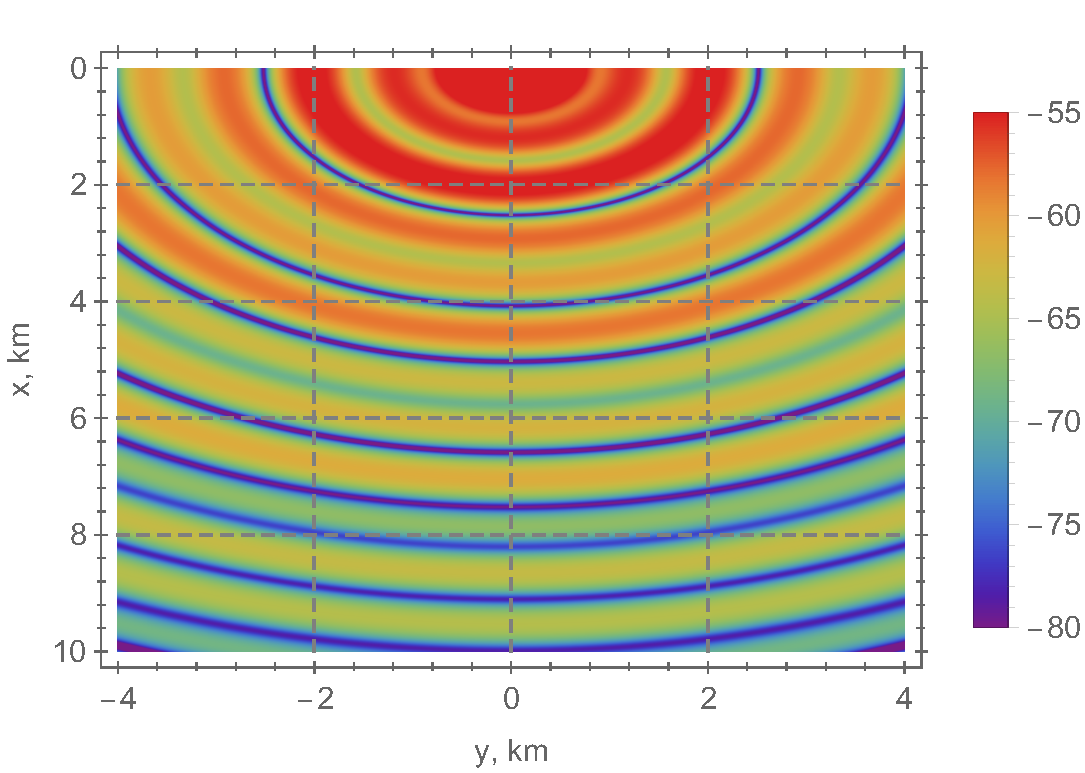
\includegraphics[width=\textwidth]{pekeris.pdf}
                        \caption{Аналитическое решение}
                    \end{subfigure}
                    \begin{subfigure}[t]{0.49\textwidth}
                        \centering
                        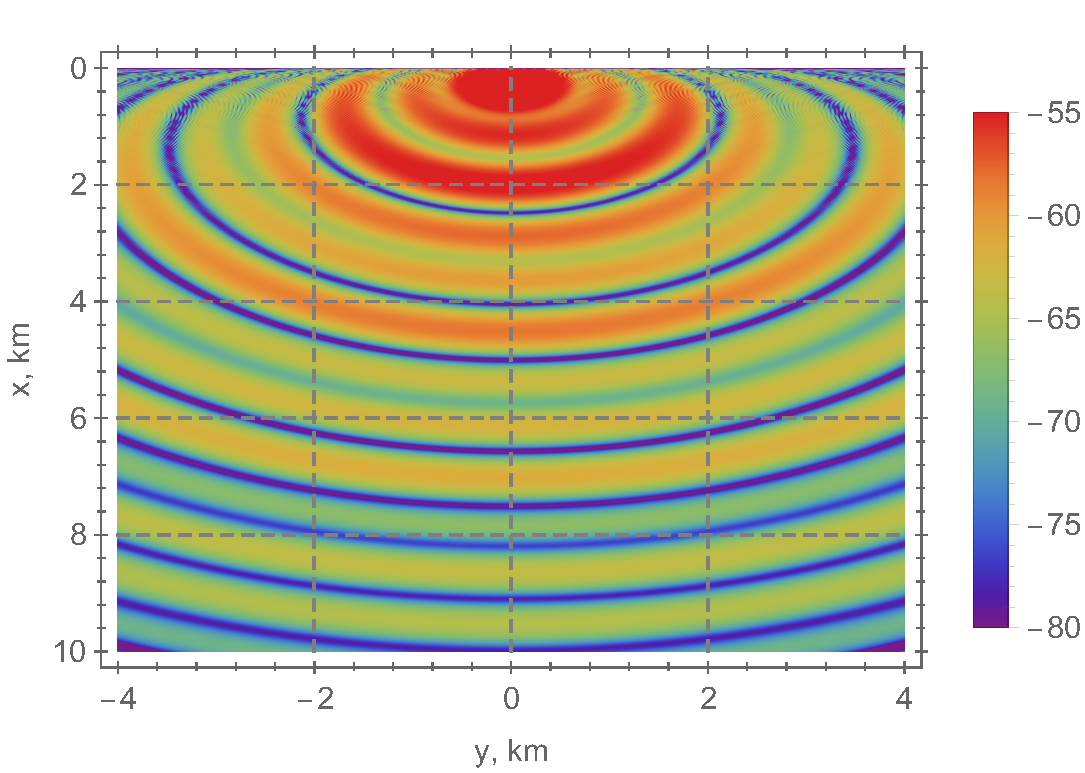
\includegraphics[width=\textwidth]{pekeris_wampe.pdf}
                        \caption{Решение \acrshort{wampe}}
                    \end{subfigure}
                    \hfill
                    \begin{subfigure}[t]{0.49\textwidth}
                        \centering
                        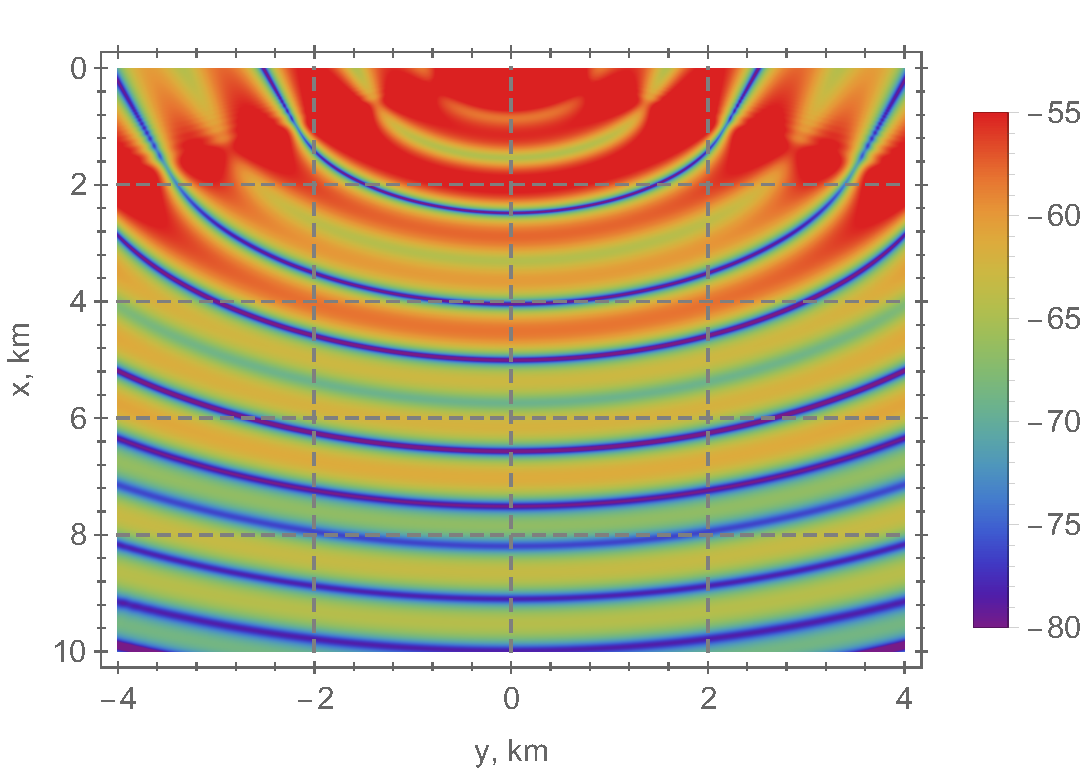
\includegraphics[width=\textwidth]{pekeris_n1.pdf}
                        \caption{\acrshort{ssp}, $p=1$}
                    \end{subfigure}
                    \begin{subfigure}[t]{0.49\textwidth}
                        \centering
                        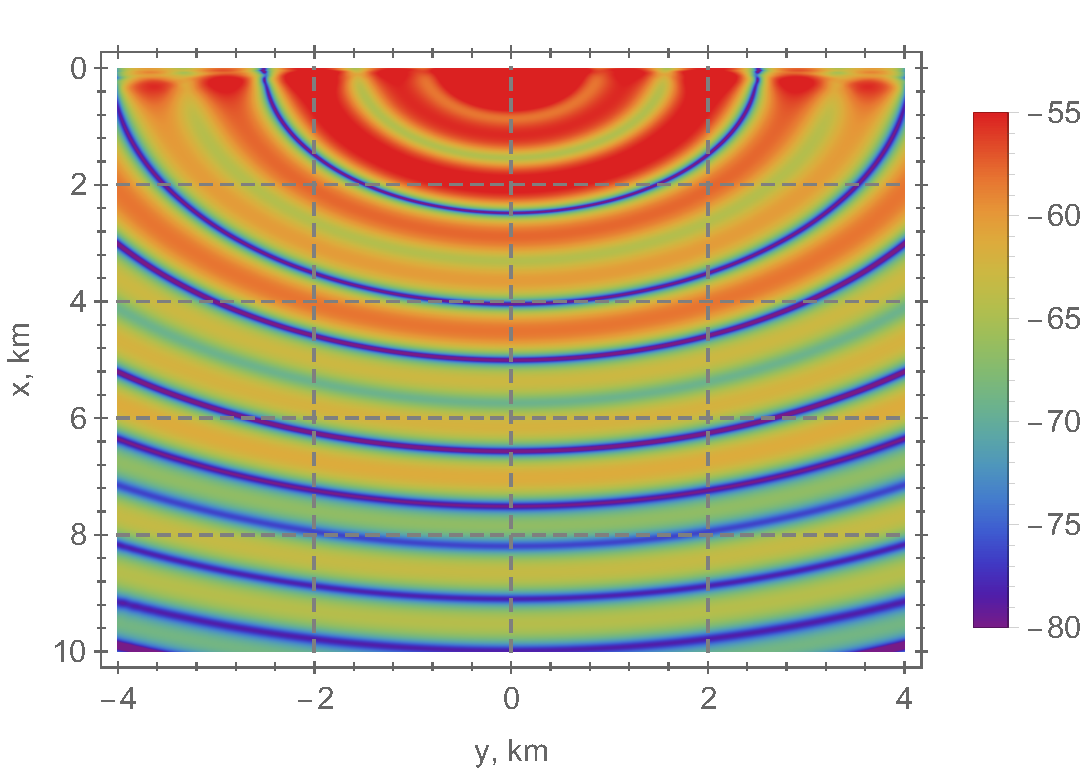
\includegraphics[width=\textwidth]{pekeris_n5.pdf}
                        \caption{\acrshort{ssp}, $p=5$}
                    \end{subfigure}
                    \hfill
                    \begin{subfigure}[t]{0.49\textwidth}
                        \centering
                        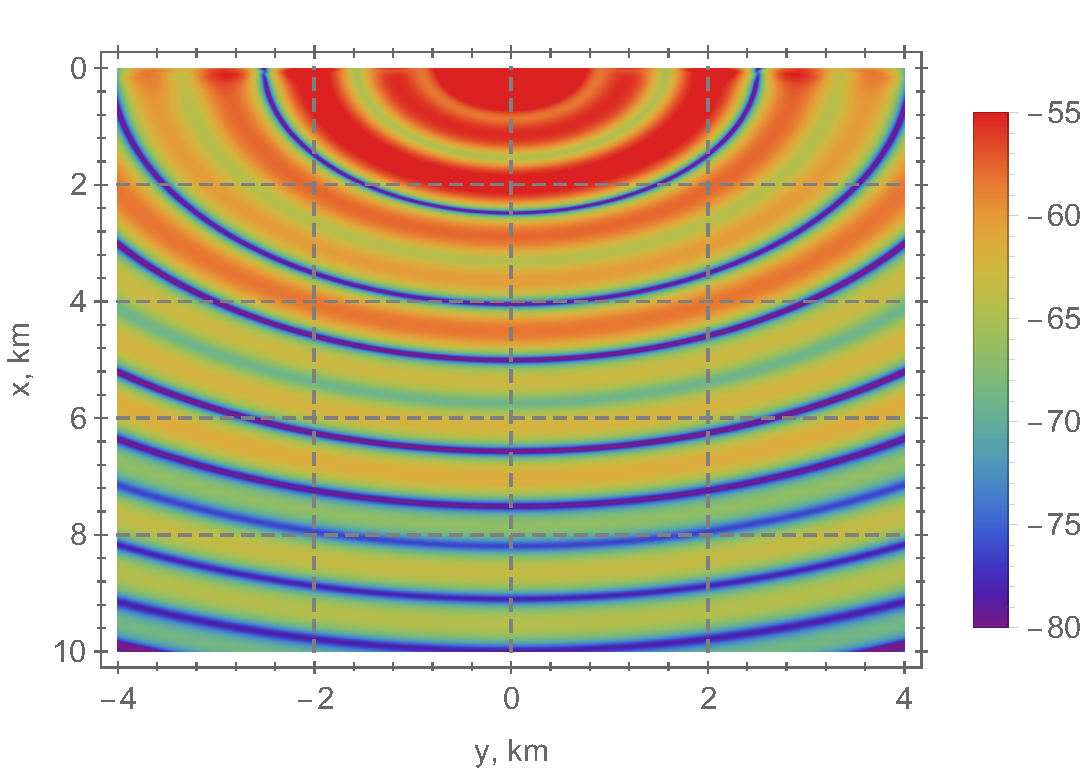
\includegraphics[width=\textwidth]{pekeris_n9.pdf}
                        \caption{\acrshort{ssp}, $p=9$}
                    \end{subfigure}
                    \begin{subfigure}[t]{0.49\textwidth}
                        \centering
                        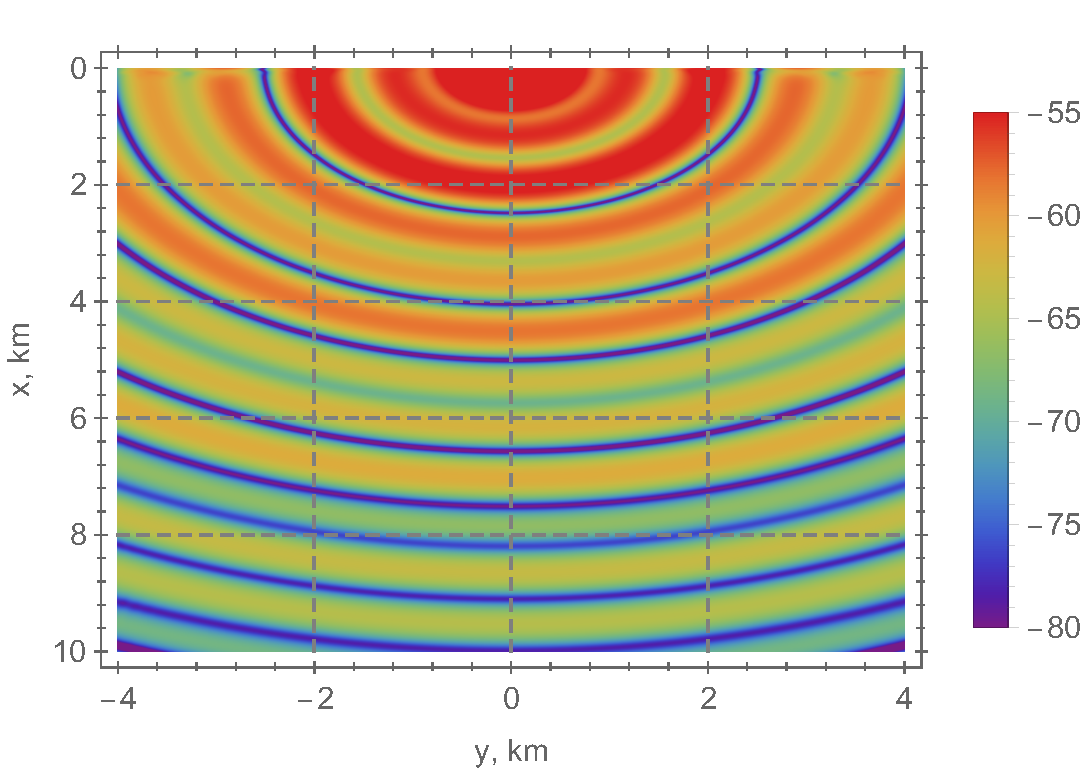
\includegraphics[width=\textwidth]{pekeris_n17.pdf}
                        \caption{\acrshort{ssp}, $p=17$}
                    \end{subfigure}
                    \caption{Акустическое поле (в дБ отн. 1 м.) в волноводе Пекериса на глубине $z=30\ \text{м.}$ с использованием лучевых начальных условий\label{fig::pekeris}}
                \end{figure}
                \begin{figure}[h]
                    \centering
                    \begin{subfigure}[t]{0.49\textwidth}
                        \centering
                        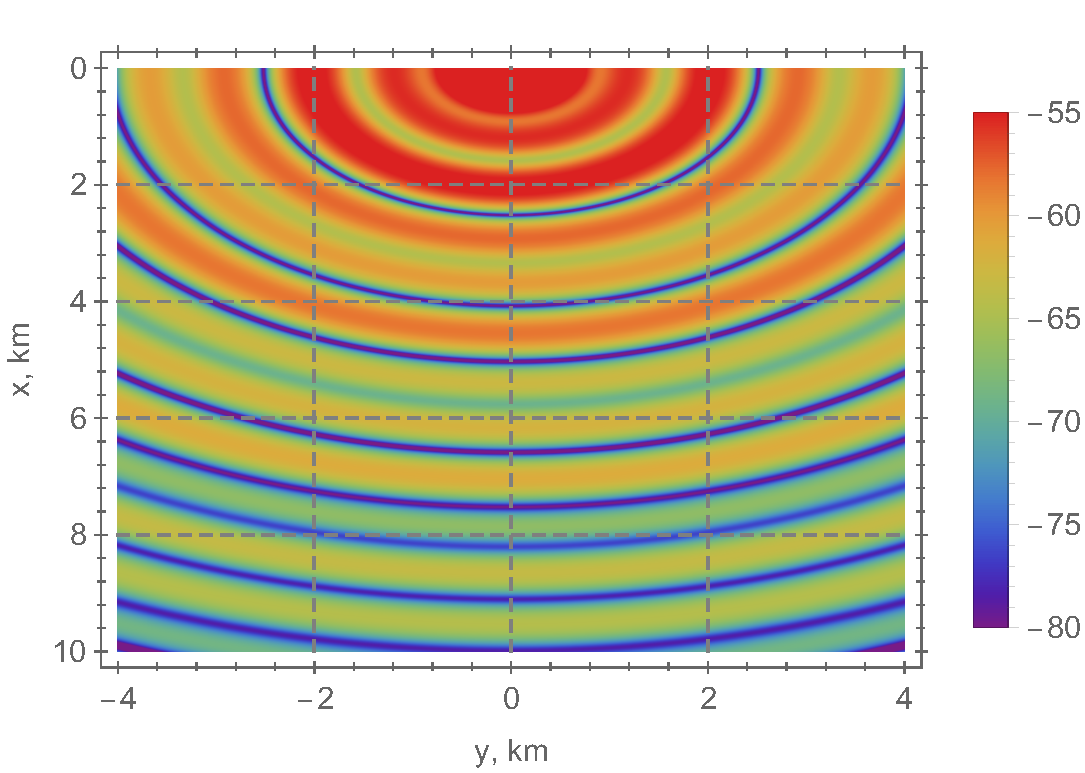
\includegraphics[width=\textwidth]{pekeris.pdf}
                        \caption{Аналитическое решение}
                    \end{subfigure}
                    \begin{subfigure}[t]{0.49\textwidth}
                        \centering
                        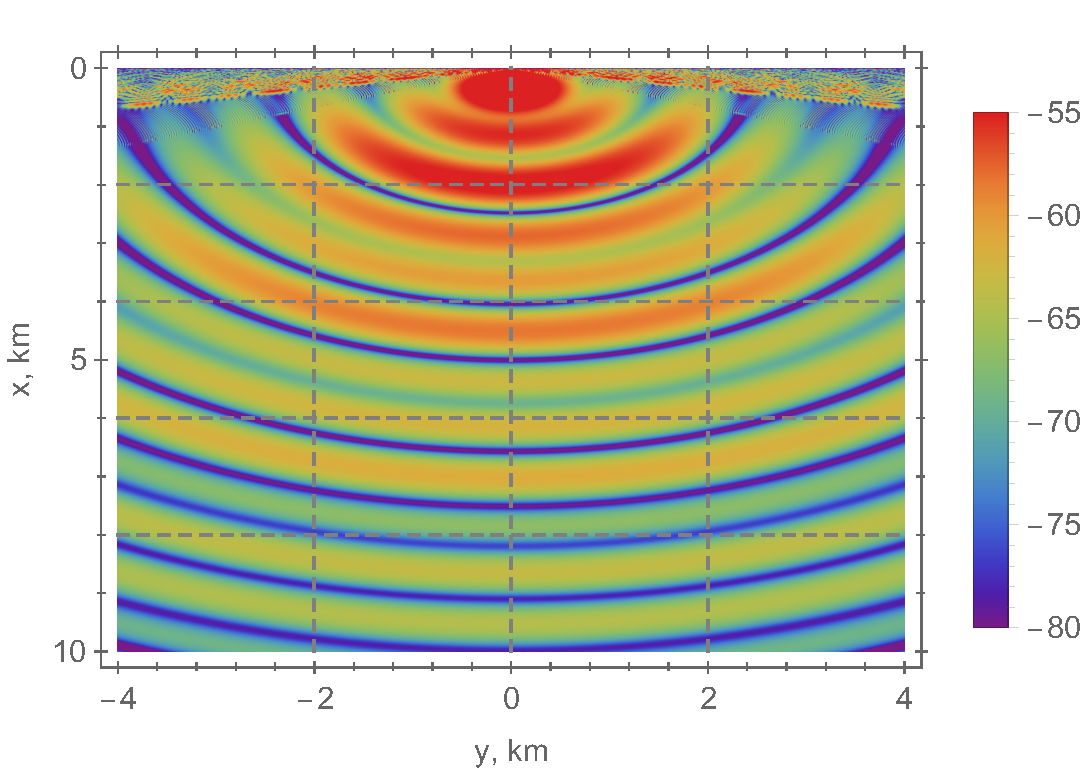
\includegraphics[width=\textwidth]{pekeris_n5_greene.pdf}
                        \caption{\acrshort{ssp}, $p=5$}
                    \end{subfigure}
                    \hfill
                    \begin{subfigure}[t]{0.49\textwidth}
                        \centering
                        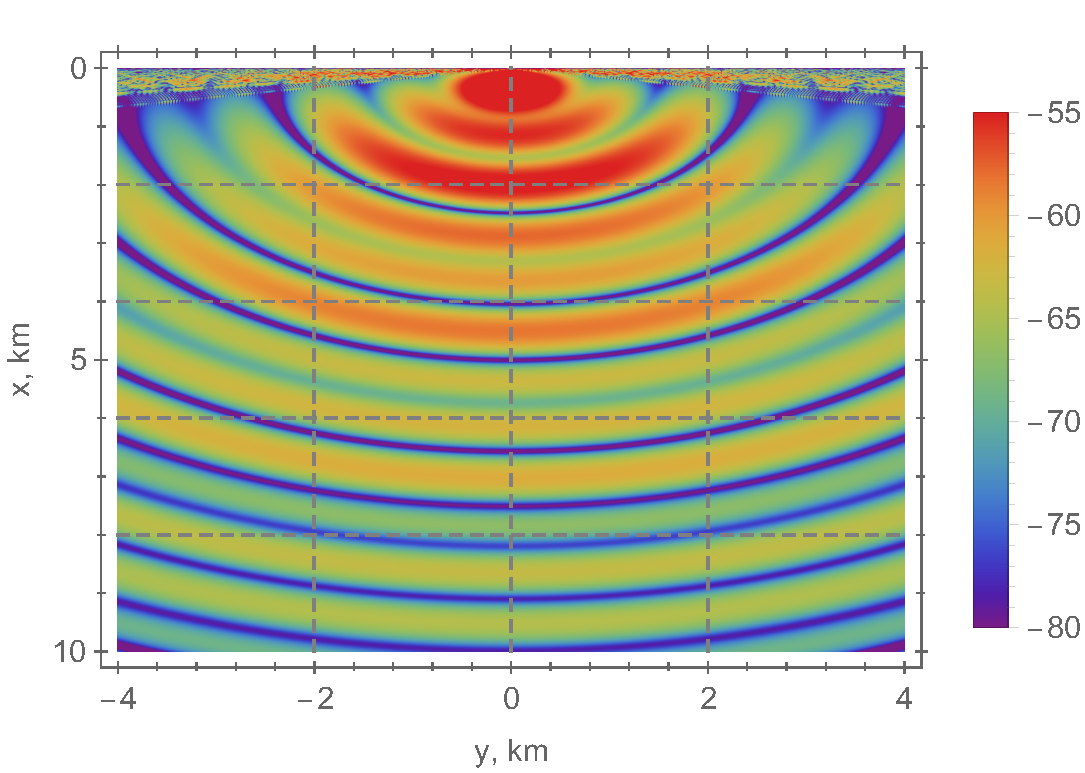
\includegraphics[width=\textwidth]{pekeris_n9_greene.pdf}
                        \caption{\acrshort{ssp}, $p=9$}
                    \end{subfigure}
                    \begin{subfigure}[t]{0.49\textwidth}
                        \centering
                        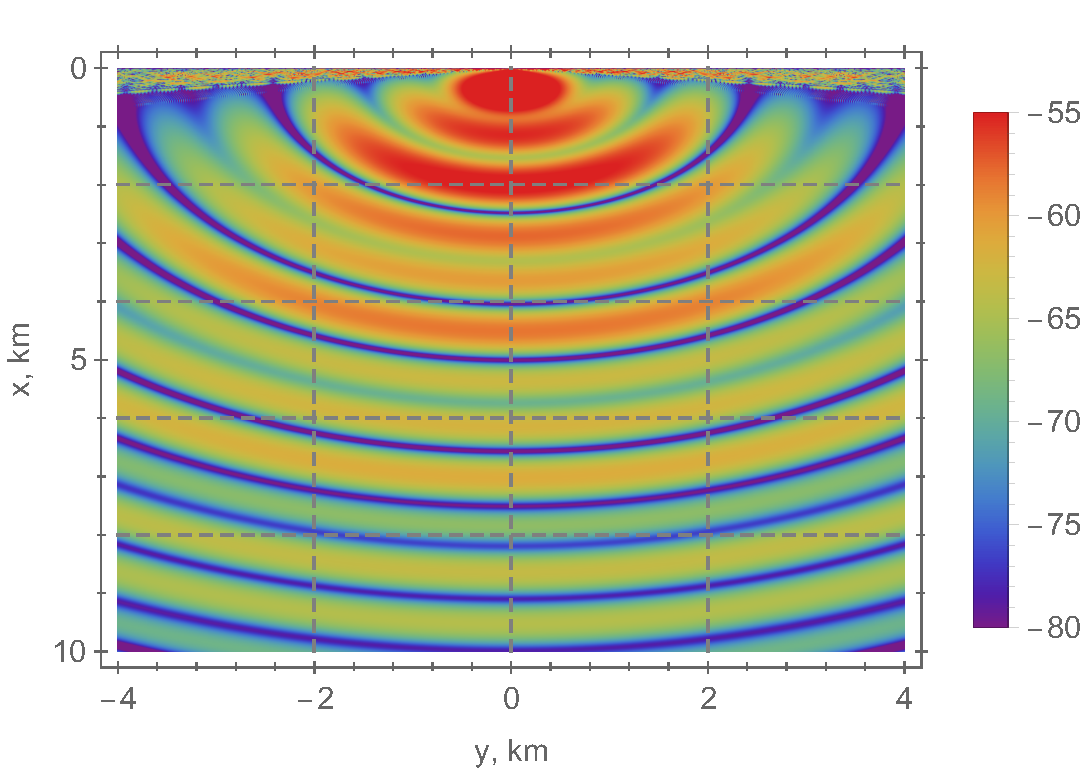
\includegraphics[width=\textwidth]{pekeris_n17_greene.pdf}
                        \caption{\acrshort{ssp}, $p=17$}
                    \end{subfigure}
                    \caption{Акустическое поле (в дБ отн. 1 м.) в волноводе Пекериса на глубине $z=30\ \text{м.}$ с использованием начального условия Грина\label{fig::pekeris_greene}}
                \end{figure}
                \begin{table}[h]
                    \centering
                    \caption{Время вычисления звукового поля в волноводе Пекериса\label{tbl::pekeris_times}}
                    \begin{tabular}{|C{3.5cm}|C{2.5cm}|C{3.5cm}|C{2.5cm}|}
                        \hline
                        Порядок аппроксимации & Время работы, с & Порядок аппроксимации & Время работы, с\\
                        \hline
                        1 & 4.6 & 9 & 15.029\\
                        \hline
                        5 & 9.624 & 17 & 25.928\\
                        \hline
                    \end{tabular}
                \end{table}
                \begin{figure}
                    \centering
                    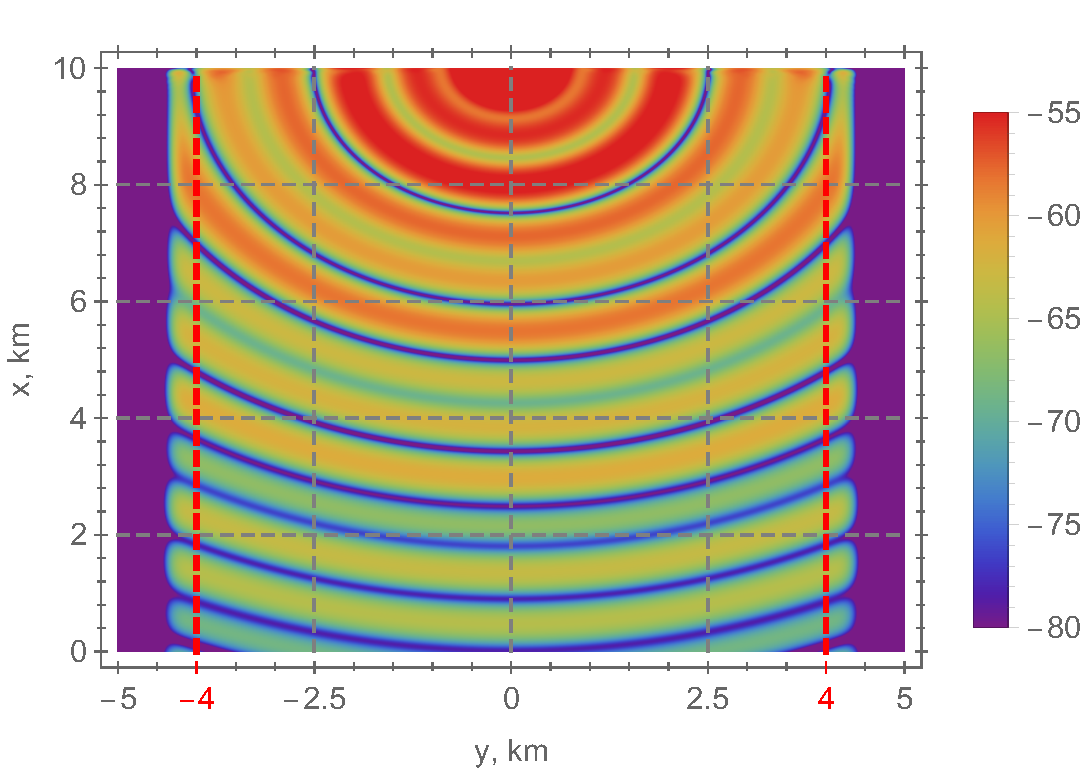
\includegraphics[width=0.6\textwidth]{pekeris_pml_n13.pdf}
                    \caption{Акустическое поле (в дБ отн. 1 м.) в волноводе Пекериса на глубине $z=30\ \text{м.}$, слои \acrshort{pml} отмечены красной пунктирной линией, ширина слоёв составляет $1000$ точек, порядок аппроксимации $p=13$\label{fig::pekeris_pml}}
                \end{figure}
                \FloatBarrier
            \subsubsection{Волновод мелкого моря с подводным каньоном}
                \par Следующим вычислительным экспериментом является моделирование распространения звуковых волн, создаваемых точечным источником в мелком море с подводным каньоном, схематическое изображение такого волновода изображено на \niceref{fig::canyon}{Рисунке}.
                \begin{figure}[h]
                    \centering
                    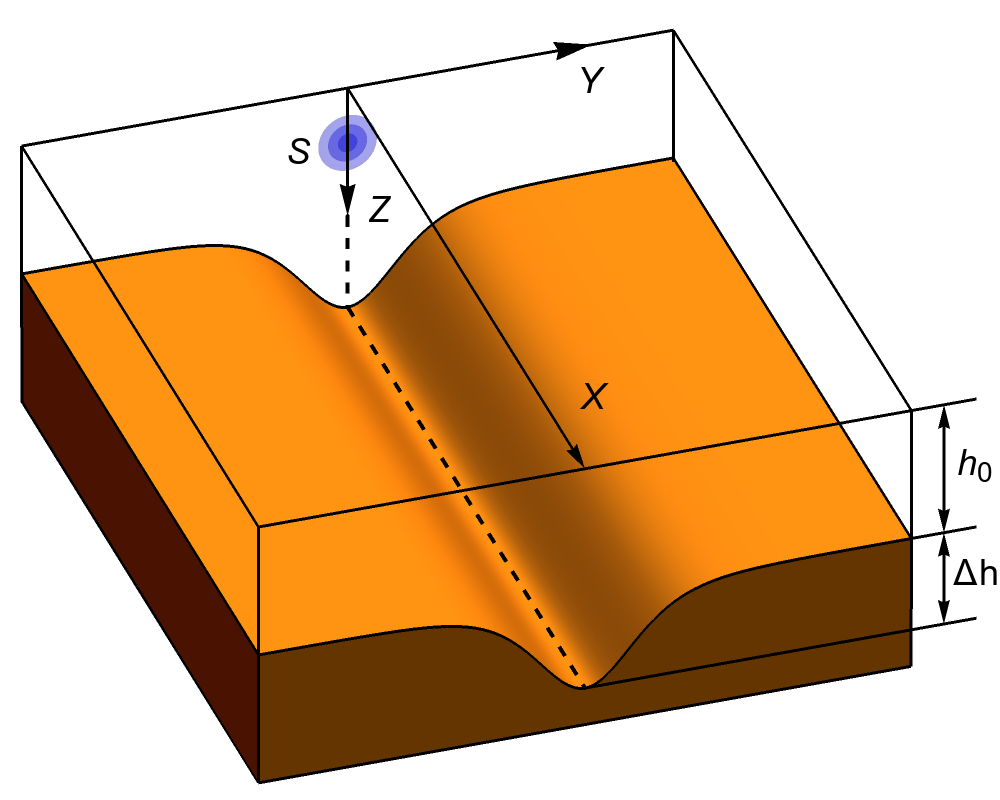
\includegraphics[width=0.5\textwidth]{canyon.png}
                    \caption{Схематическое изображение подводного каньона\label{fig::canyon}}
                \end{figure}
                Рельеф дна описывается функцией
                \begin{equation}
                    z=h\pa{y}=h_0+\Delta h\sech^2\pa{\sigma y}\,.
                \end{equation}
                \par В данном эксперименте были использованы следующие параметры
                \begin{equation}
                    \begin{array}{ccc}
                        h_0=50\ \text{м}\,, & \Delta h=5\ \text{м}\,, & \sigma=0.005\,,\\
                        z_s=10\ \text{м}\,, & p=11\,, & \alpha\approx\pm86^\circ\,,\\
                        x_0=50\ \text{м}\,, & x_1=30\ \text{км}\,, & n_x=30001\,,\\
                        y_0=-1\ \text{км}\,, & y_1=1\ \text{км}\,, & n_y=2001\,,
                    \end{array}
                \end{equation}
                при которых на частоте $f=120\ \text{Гц}$ имеются четыре захваченные моды. Звуковое поле было вычислено с порядком аппроксимации $p=11$, результаты вычислений отображены на \niceref{fig::canyon_field}{Рисунке}, время вычисления составило $22.791\ \text{с}$. На рисунках хорошо видно, как звук фокусируется в каньоне. Решение, полученное предыдущей версией программы почти не отличается от решения, полученного методом \acrshort{ssp}, что подтверждает теорию о том, что в рамках данной задачи апертура уравнения играет незначительное роль. На \niceref{fig::canyon_compare}{Рисунке} полученное решение сравнивается с решением трёхмерного параболического уравнения \cite{isakson14,lin12,shtrum16}. Из рисунка видно, что решения достаточно сильно совпадают, как и в случае с широкоугольным параболическим уравнением \cite{bachelor}.
                \begin{figure}[h]
                    \centering
                    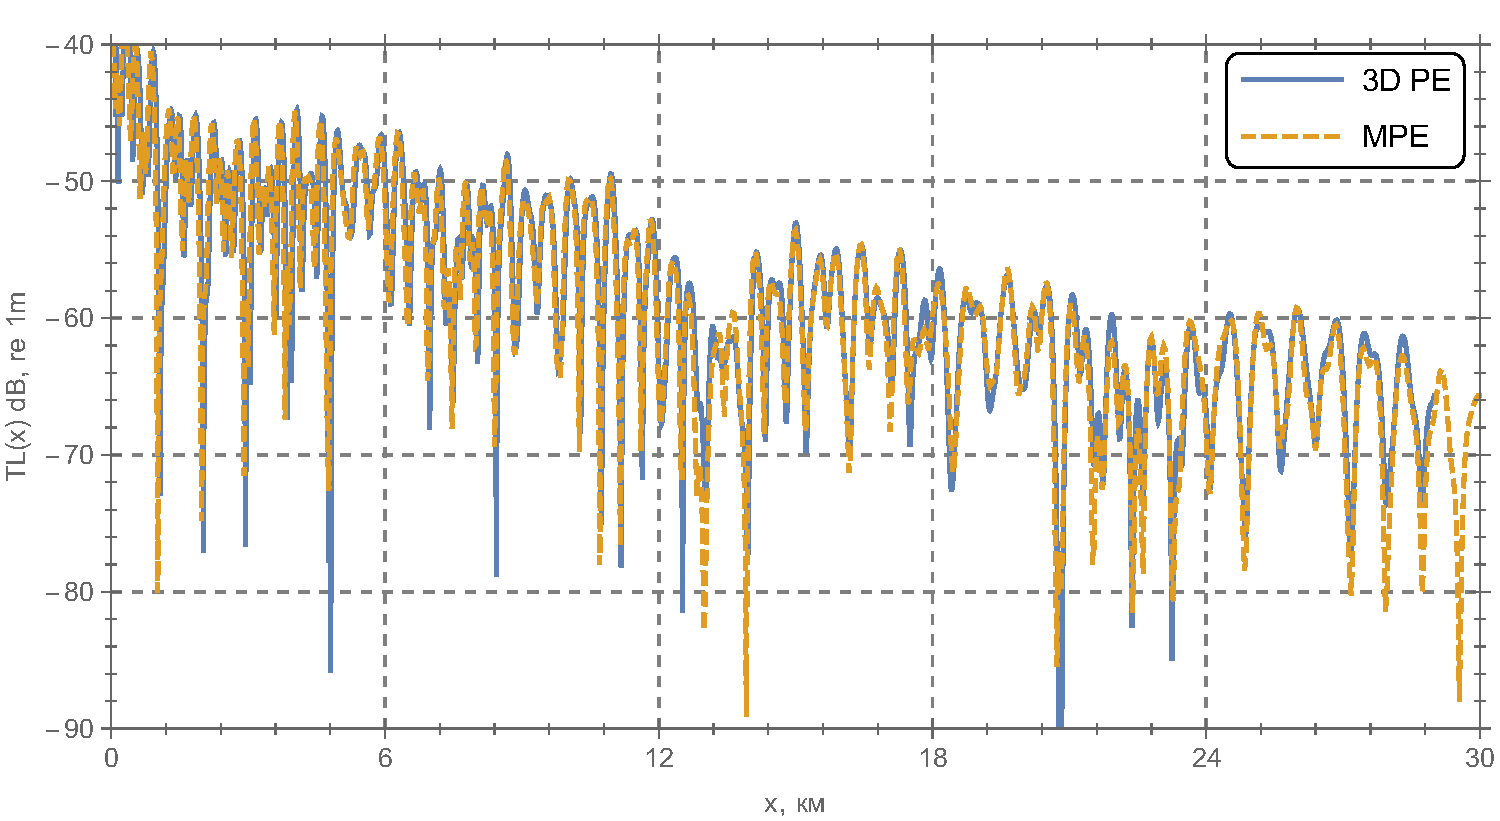
\includegraphics[width=0.9\textwidth]{canyon_compare.pdf}
                    \caption{Сравнение результатов вычисления акустического поля (в дБ отн. 1 м.) в мелком море с подводным каньоном при $y=0\ \text{км.}$ на глубине $z=10\ \text{м}$.\label{fig::canyon_compare}}
                \end{figure}
                \begin{figure}[h]
                    \centering
                    \begin{subfigure}[t]{0.75\textwidth}
                        \centering
                        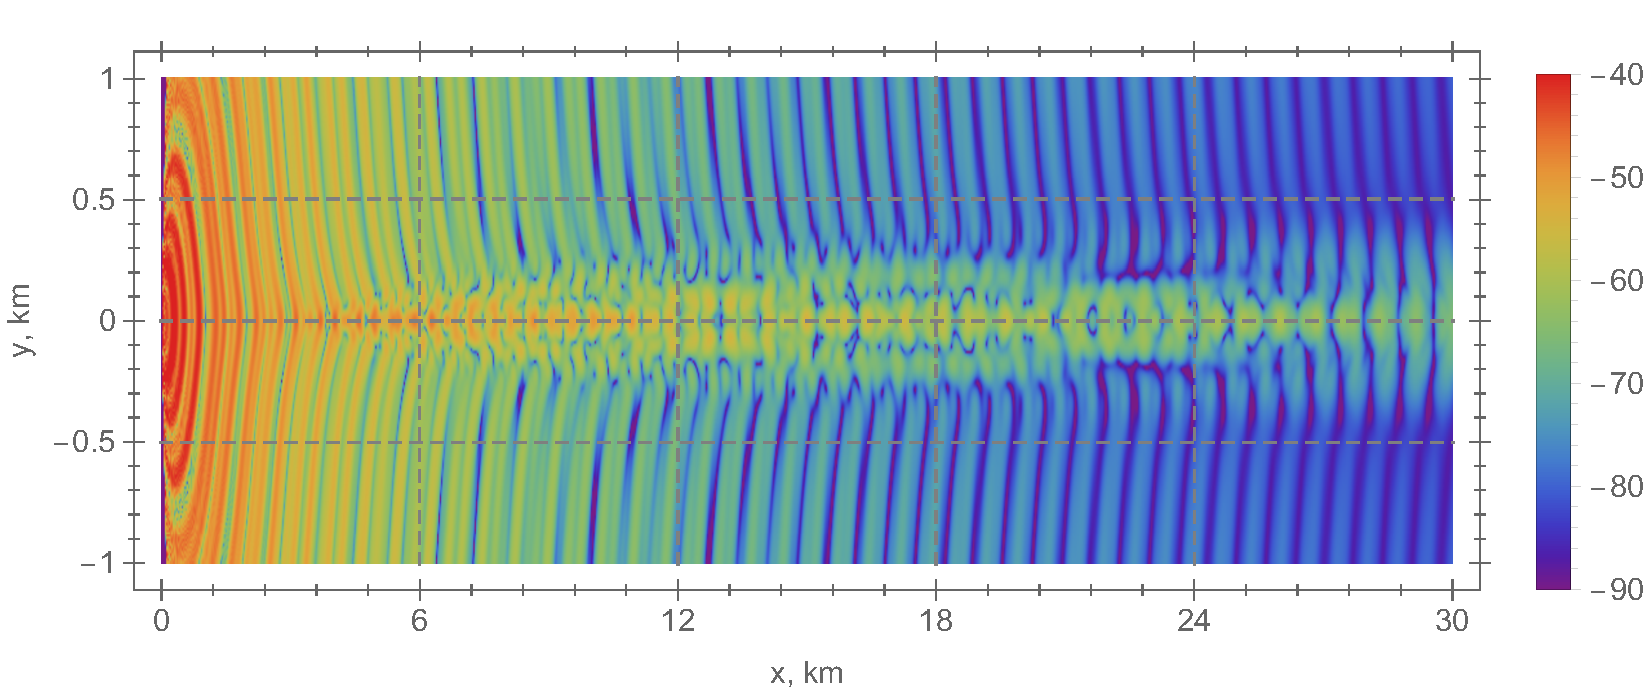
\includegraphics[width=\textwidth]{canyon_wampe.pdf}
                        \caption{Решение \acrshort{wampe}, $z=10\ \text{м}$}
                    \end{subfigure}
                    \hfill
                    \begin{subfigure}[t]{0.75\textwidth}
                        \centering
                        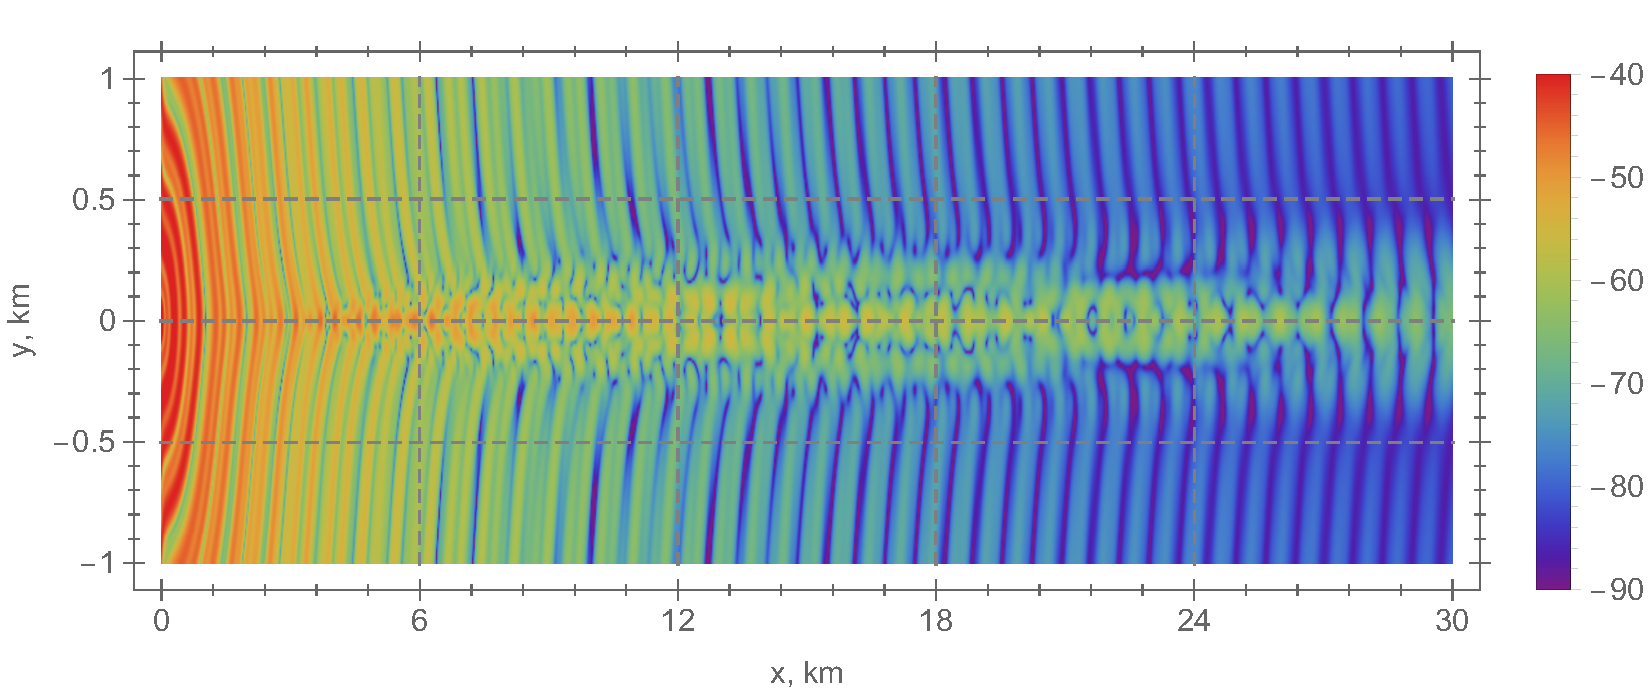
\includegraphics[width=\textwidth]{canyon_n11.pdf}
                        \caption{\acrshort{ssp}, $z=10\ \text{м}$}
                    \end{subfigure}
                    \hfill
                    \begin{subfigure}[t]{0.75\textwidth}
                        \centering
                        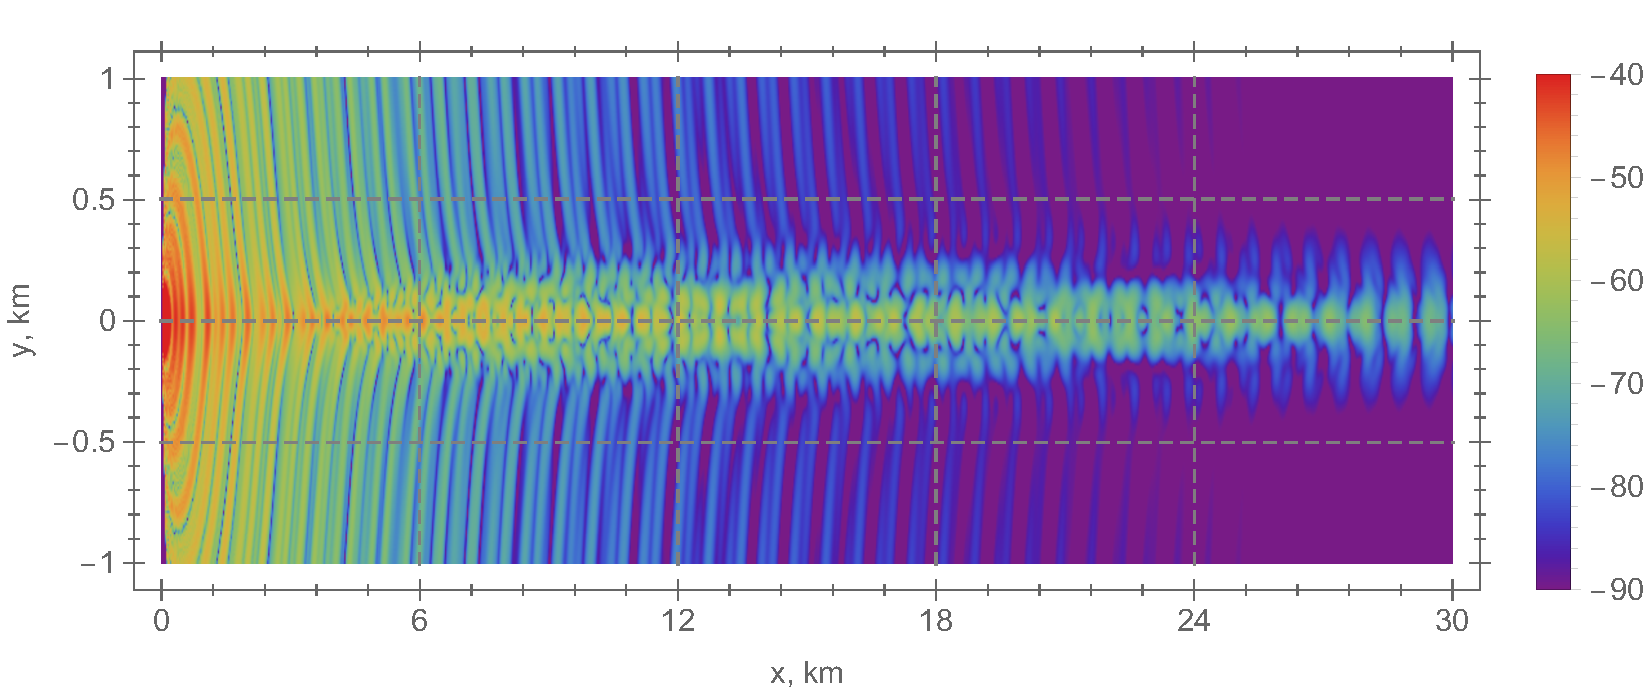
\includegraphics[width=\textwidth]{canyon_wampe_deep.pdf}
                        \caption{Решение \acrshort{wampe}, $z=55\ \text{м}$}
                    \end{subfigure}
                    \hfill
                    \begin{subfigure}[t]{0.75\textwidth}
                        \centering
                        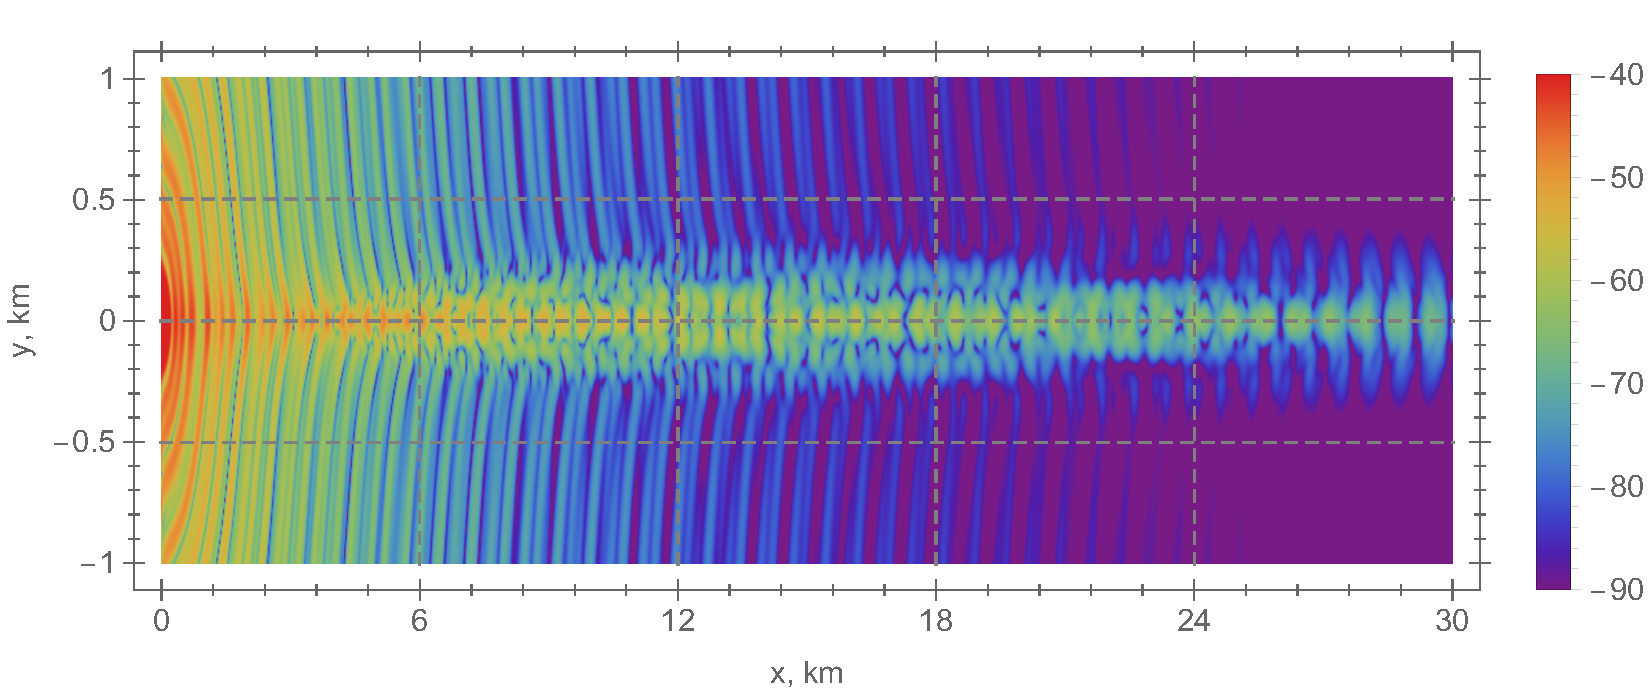
\includegraphics[width=\textwidth]{canyon_n11_deep.pdf}
                        \caption{\acrshort{ssp}, $z=55\ \text{м}$}
                    \end{subfigure}
                    \caption{Акустическое поле (в дБ отн. 1 м.) в клиновидном волноводе\label{fig::canyon_field}}
                \end{figure}
                \FloatBarrier
            \subsubsection{Клиновидный волновод мелкого моря}
                \par Следующий вычислительный эксперимент было проведён для моделирования распространения звуковых волн в мелком море с подводным клином. Схематическое изображение этого волновода дано на
                \begin{figure}[h]
                    \centering
                    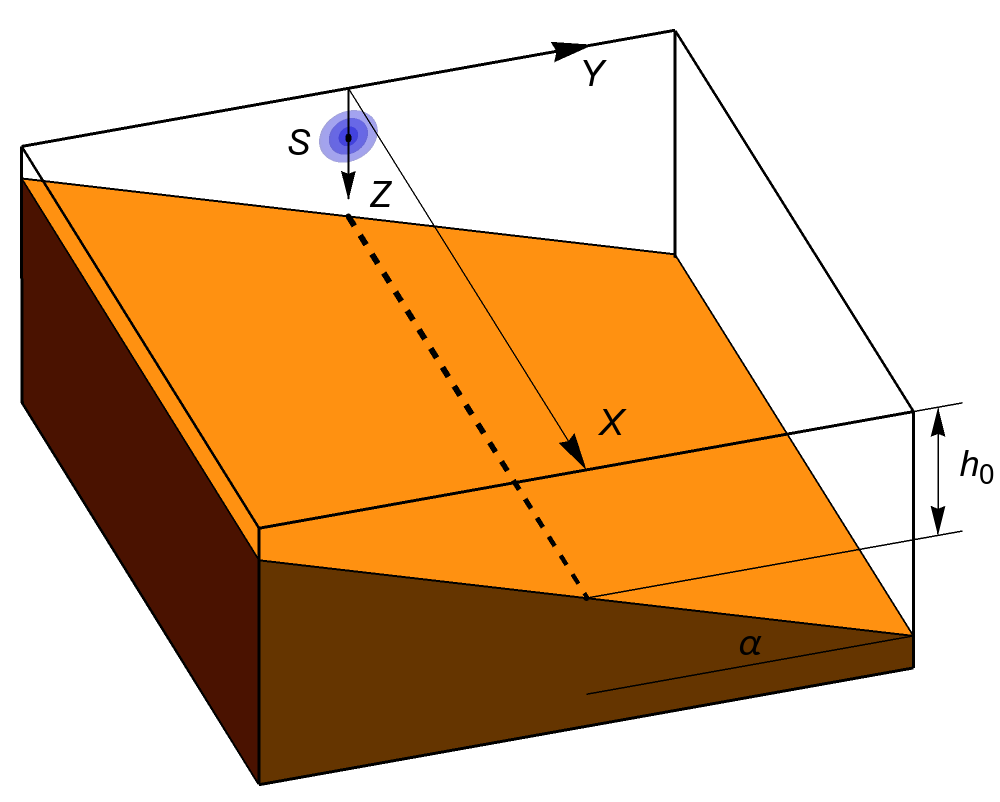
\includegraphics[width=0.5\textwidth]{wedge.png}
                    \caption{Схематическое изображение подводного каньона\label{fig::wedge}}
                \end{figure}
                Рельеф дна задаётся функцией
                \begin{equation}
                    z=h\pa{y}=h_0+y\tan\beta\,.
                \end{equation}
                \par Точечный источник расположен достаточно далеко от вершины клина на глубине $z=z_s$. Акустическое поле было вычислено на глубине $z=30\ \text{м}$ и были использованы следующие параметры
                \begin{equation}
                    \begin{array}{ccc}
                        z_s=100\ \text{м}\,,&h_0=200\ \text{м}\,,&\beta\approx2.86^\circ\,,\\
                       f=25\ \text{Гц}\,,&p=13\,,&\alpha=\pm89.95^\circ\,,\\
                       x_0=50\ \text{м}\,,&x_1=25\ \text{км}\,,&n_x=50001\,,\\
                       y_0=-3.32\ \text{км}\,,&y_1=3.32\ \text{км}\,,&n_y=13282\,.
                    \end{array}
                \end{equation}
                \par Результат вычислений показан на \niceref{fig::wedge_field}{Рисунке}, время работы программы составило $173.386\ \text{с}$. В целом решения \acrshort{wampe} и \acrshort{ssp} похожи, однако даже на значительно расстоянии от источника заметна более широкая апертура \acrshort{ssp} решения. Так как используемая модель не учитывает взаимодействия мод, звуковое поле обрезается, ввиду того, что при уменьшении глубины дна пропадают моды старших порядков. На \niceref{fig::wedge_comp}{Рисунке} показано сравнение решений при различных координатах $x$, из которого видно, что вблизи источника \acrshort{ssp} решение не образует численного шума, а при отдалении от источника становится заметна более широкая апертура этого решения. Также было проведено сравнение с решением методом изображений \cite{deane,tang}. Как показано на \niceref{fig::wedge_compare}{Рисунке}, решения всех методов почти совпадают, не смотря на адиабатическую природу модовых параболических уравнений, при этом большая апертура \acrshort{ssp} метода ещё сильнее приближает решение к решению методом изображений вдали от источника.
                \begin{figure}[h]
                    \centering
                    \begin{subfigure}[t]{0.49\textwidth}
                        \centering
                        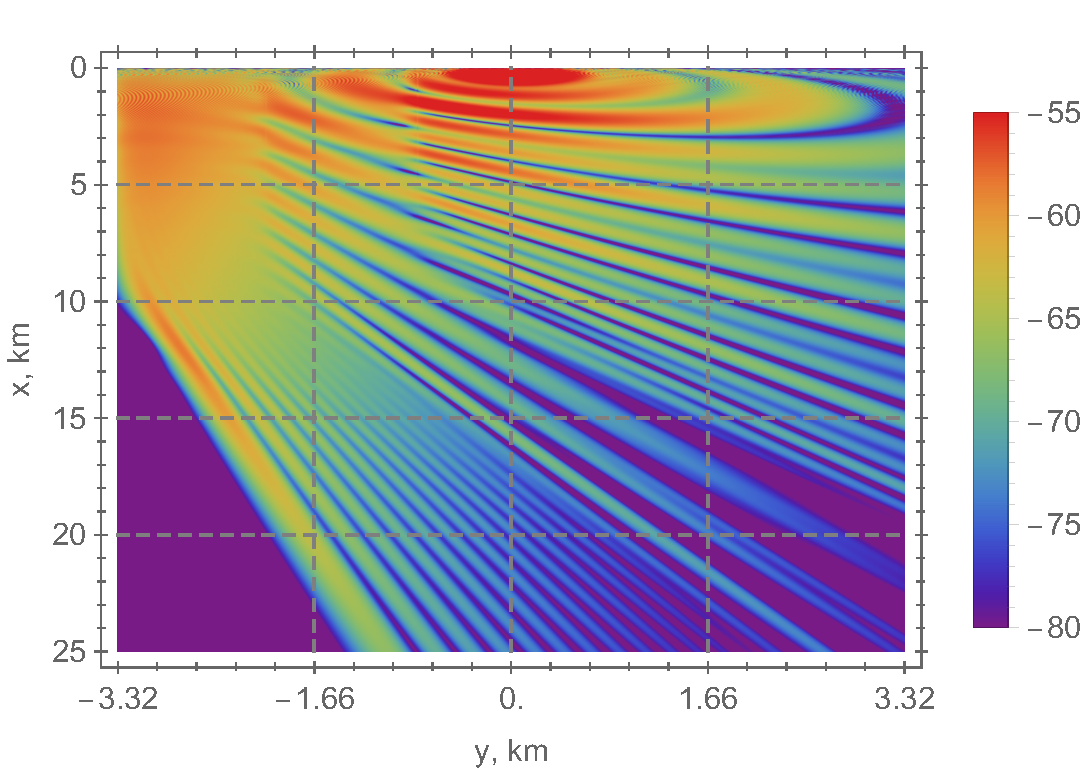
\includegraphics[width=\textwidth]{wedge_wampe.pdf}
                        \caption{Решение \acrshort{wampe}}
                    \end{subfigure}
                    \begin{subfigure}[t]{0.49\textwidth}
                        \centering
                        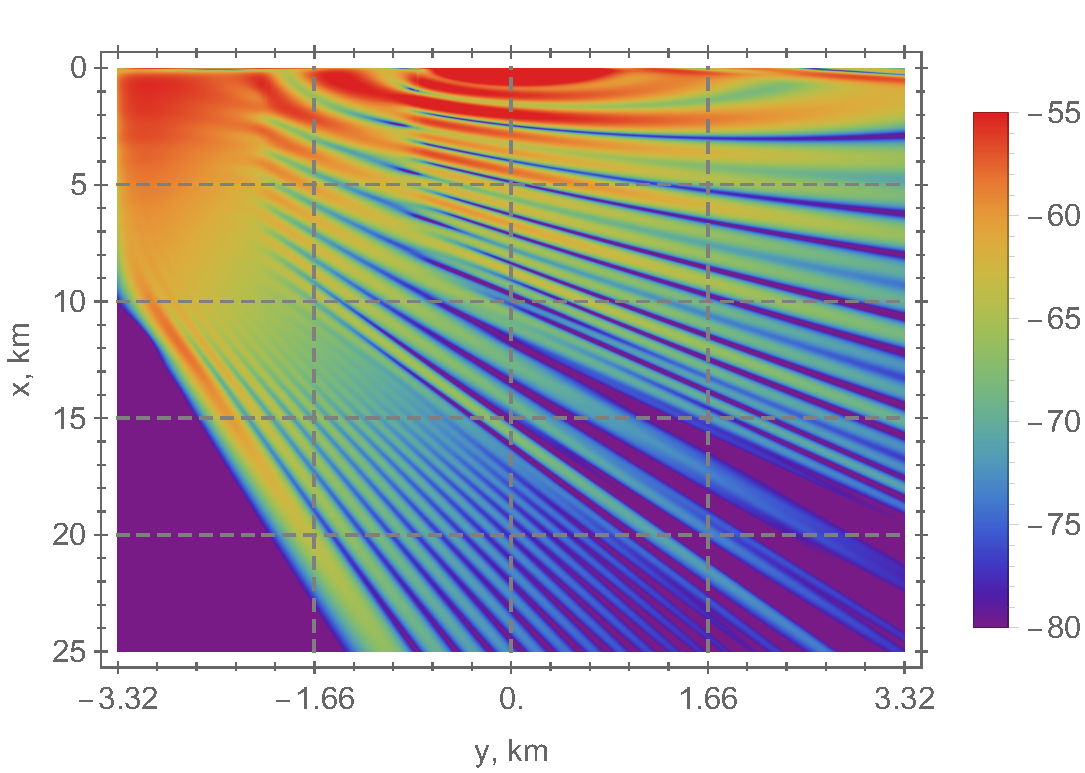
\includegraphics[width=\textwidth]{wedge_n13.pdf}
                        \caption{\acrshort{ssp}}
                    \end{subfigure}
                    \hfill
                    \caption{Акустическое поле (в дБ отн. 1 м.) в мелком море с подводным клином $z=30\ \text{м.}$\label{fig::wedge_field}}
                \end{figure}
                \begin{figure}[h]
                    \centering
                    \begin{subfigure}[t]{0.9\textwidth}
                        \centering
                        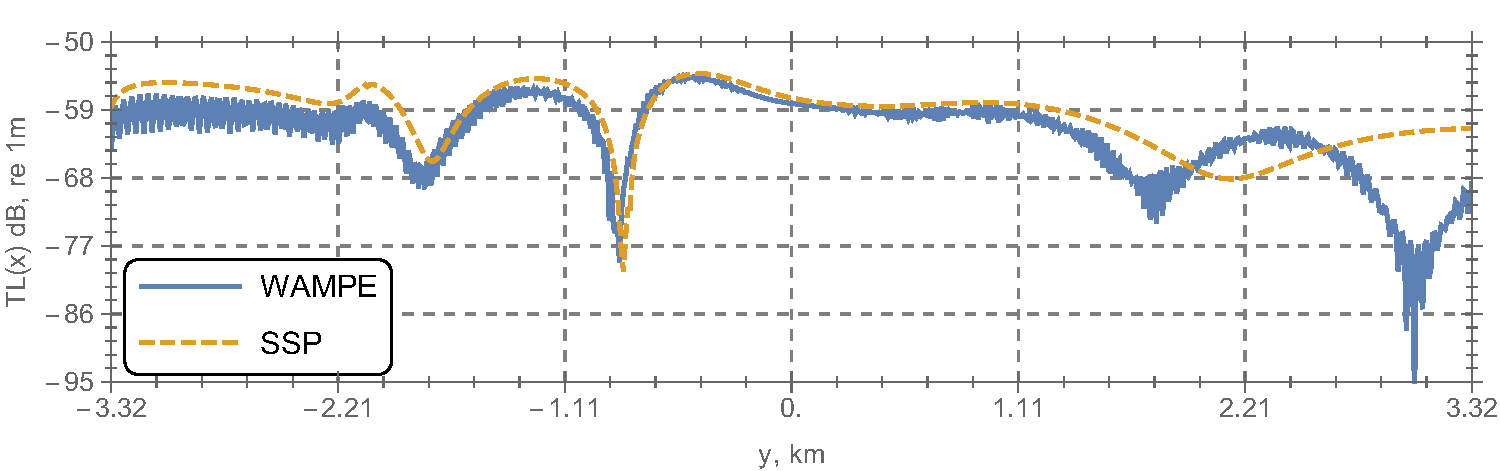
\includegraphics[width=\textwidth]{wedge_comp_1.pdf}
                        \caption{$x_c=1\ \text{км.}$}
                    \end{subfigure}
                    \hfill
                    \begin{subfigure}[t]{0.9\textwidth}
                        \centering
                        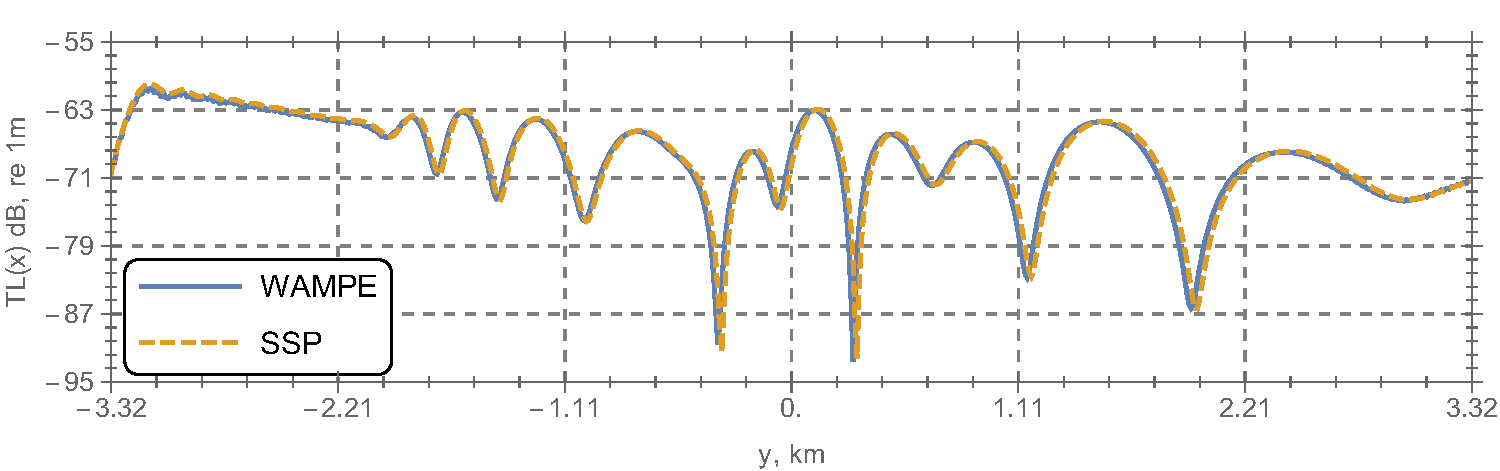
\includegraphics[width=\textwidth]{wedge_comp_9.pdf}
                        \caption{$x_c=9\ \text{км.}$}
                    \end{subfigure}
                    \hfill
                    \begin{subfigure}[t]{0.9\textwidth}
                        \centering
                        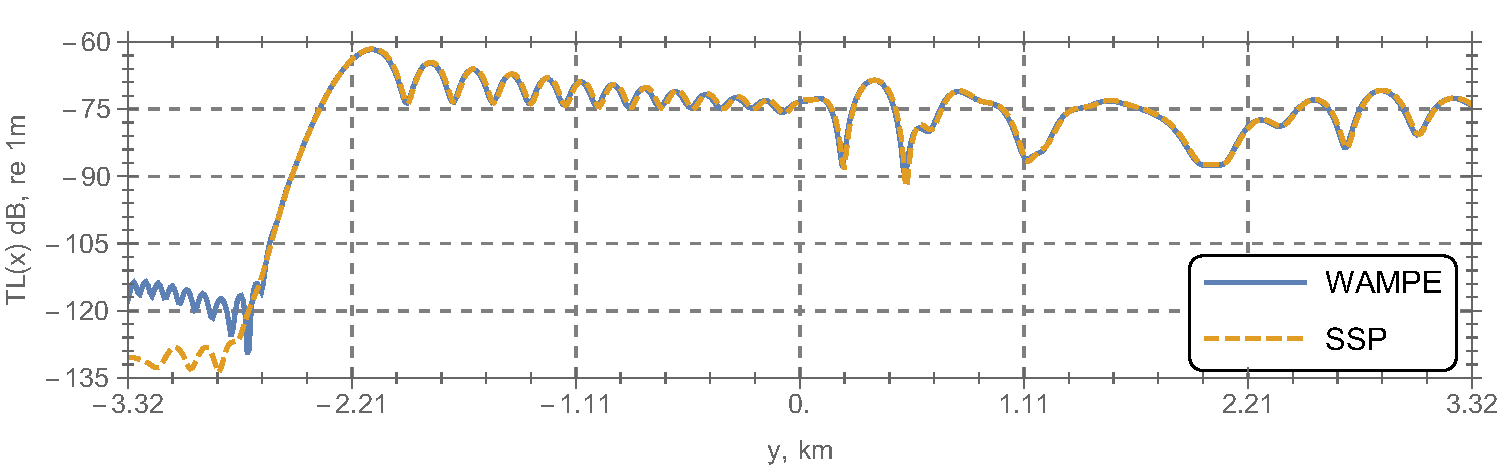
\includegraphics[width=\textwidth]{wedge_comp_17.pdf}
                        \caption{$x_c=17\ \text{км.}$}
                    \end{subfigure}
                    \hfill
                    \begin{subfigure}[t]{0.9\textwidth}
                        \centering
                        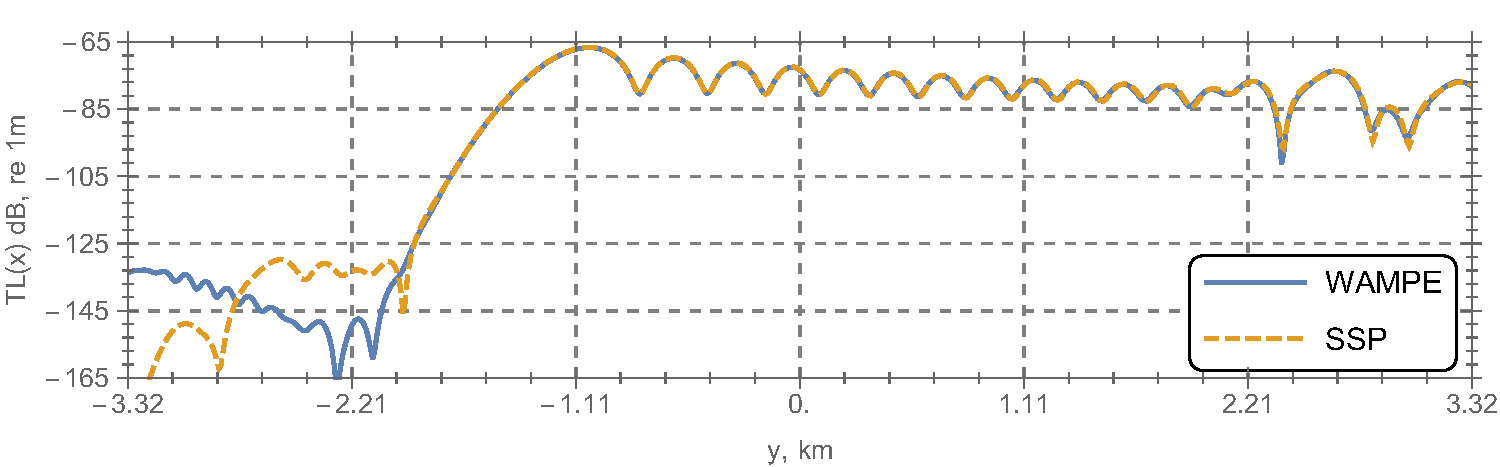
\includegraphics[width=\textwidth]{wedge_comp_25.pdf}
                        \caption{$x_c=25\ \text{км.}$}
                    \end{subfigure}
                    \caption{Сравнение результатов вычисления акустического поля (в дБ отн. 1 м.) в мелком море с подводным клином при $x=x_c$\label{fig::wedge_comp}}
                \end{figure}
                \begin{figure}[h]
                    \centering
                    \begin{subfigure}[t]{0.9\textwidth}
                        \centering
                        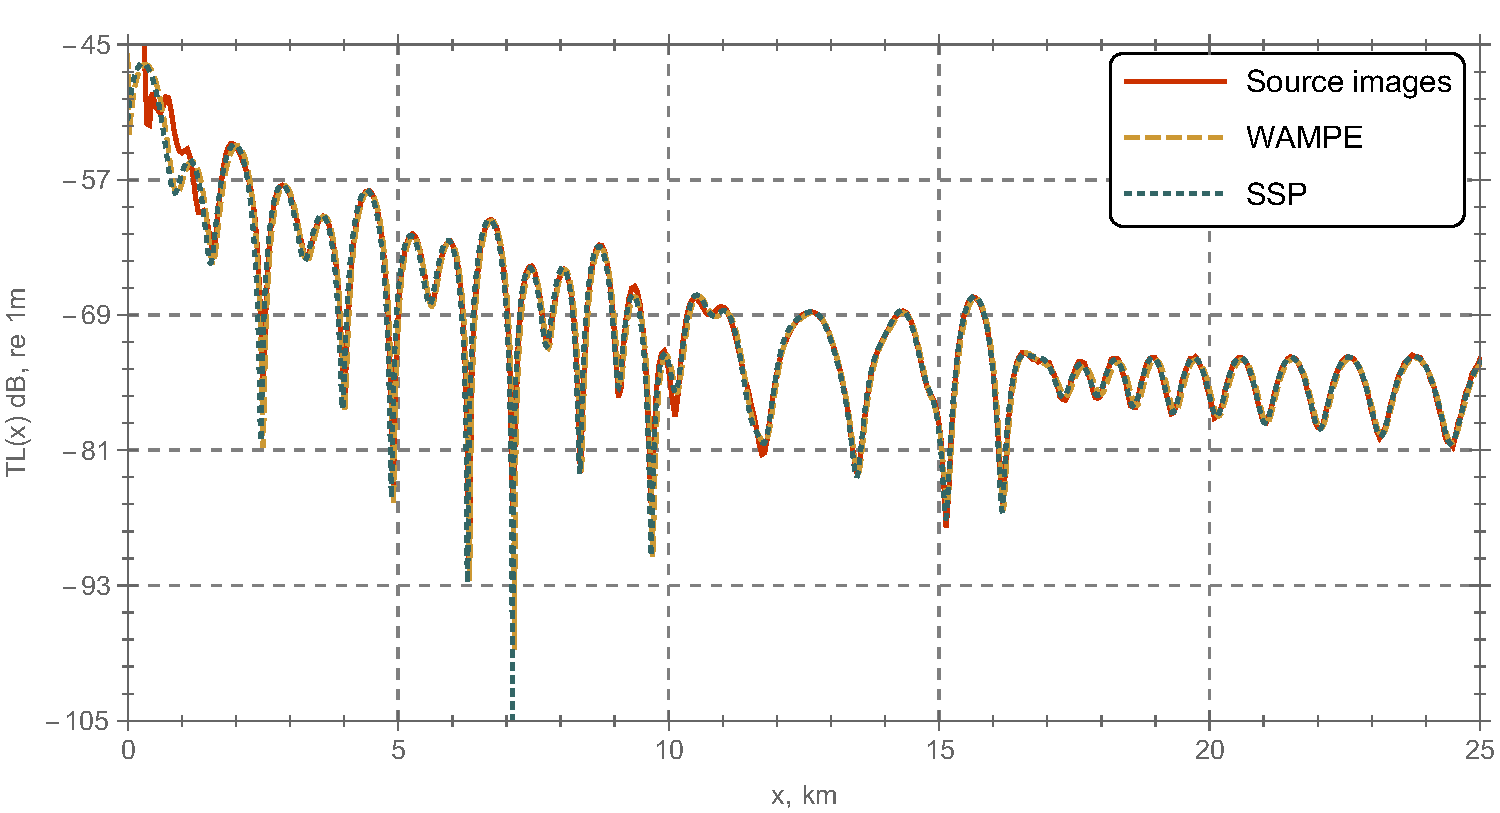
\includegraphics[width=0.9\textwidth]{wedge_comp.pdf}
                    \end{subfigure}
                    \hfill
                    \begin{subfigure}[t]{0.9\textwidth}
                        \centering
                        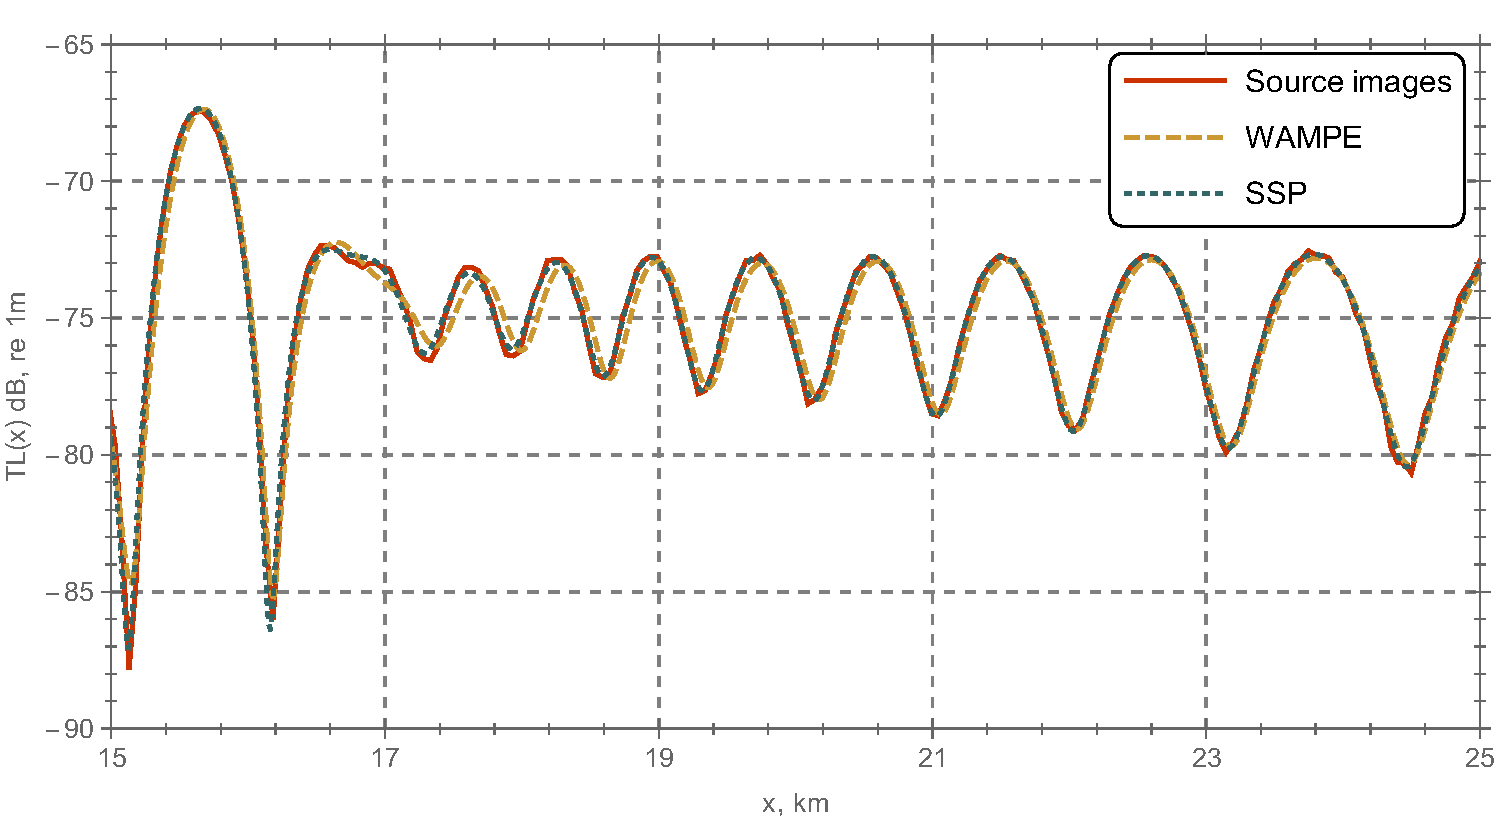
\includegraphics[width=0.9\textwidth]{wedge_comp_close.pdf}
                    \end{subfigure}
                    \caption{Сравнение результатов вычисления акустического поля (в дБ отн. 1 м.) в мелком море с подводным клином при $y=0\ \text{км}$.\label{fig::wedge_compare}}
                \end{figure}
                \FloatBarrier
            \subsubsection{Волновод с реальной батиметрией}
                \par В качестве последнего эксперимента было проведено моделирование распространения звуковых волн в волноводе с использованием реальных данных батиметрии, рельеф дна которого изображён на \niceref{fig::sakhalin}{Рисунке}.
                \begin{figure}[h]
                    \centering
                    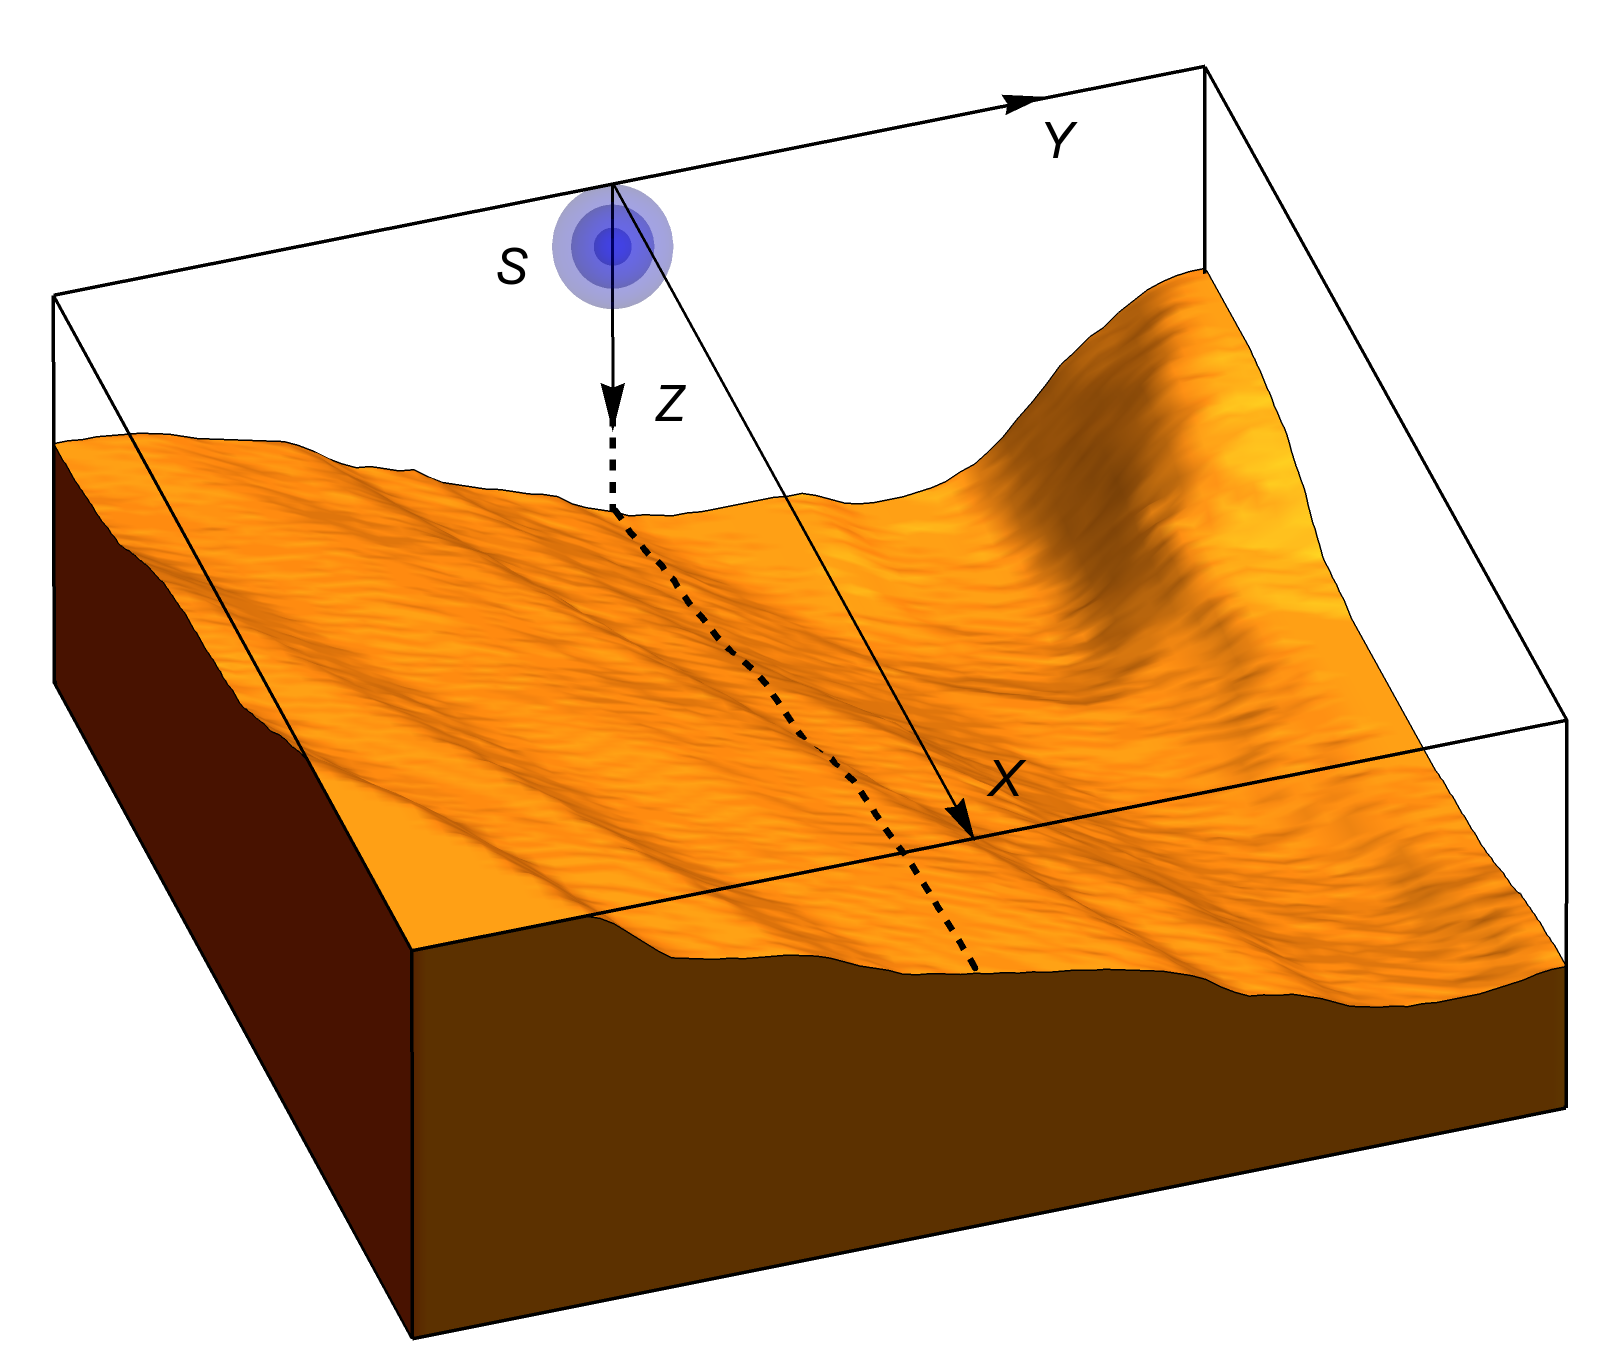
\includegraphics[width=0.5\textwidth]{sakhalin.png}
                    \caption{Изображение волновода с реальной батиметрией\label{fig::sakhalin}}
                \end{figure}
                \begin{figure}[h]
                    \centering
                    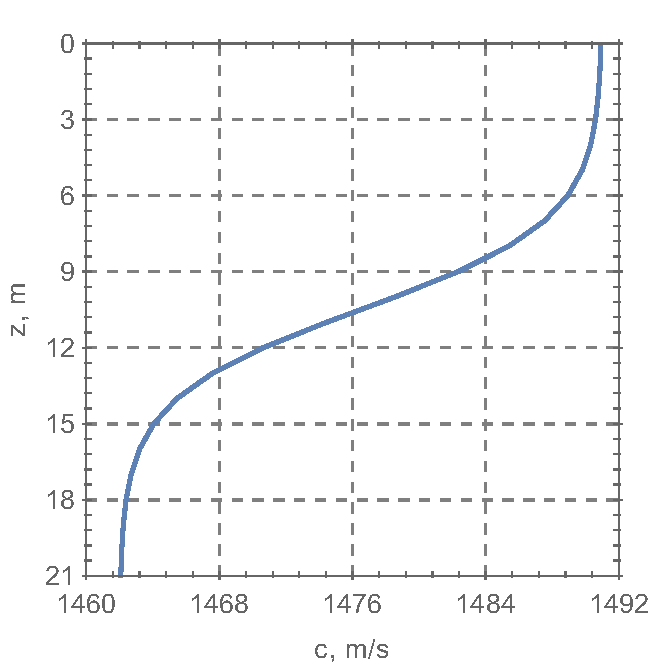
\includegraphics[width=0.5\textwidth]{sound_profile.pdf}
                    \caption{Изображение профиля скорости звука\label{fig::sakhalin_sound_profile}}
                \end{figure}
                Также был использован профиль скорости звука в воде, изображённый на \niceref{fig::sakhalin_sound_profile}{Рисунке} и задаётся формулой
                \begin{equation}
                    c\pa{z}=-\frac{29}{1+e^{-\pa{\frac{12z}{21}-6}}}+1491\,.
                \end{equation}
                \par При проведении эксперимента было вычислено акустическое поле источника, расположенного на глубине $z=z_s=4\ \text{м}$, и были использованы следующие параметры
                \begin{equation}
                    \begin{array}{ccc}
                        f=150\ \text{Гц}\,,&p=11\,,&\alpha=\pm89.95^\circ\,,\\
                        x_0=50\ \text{м}\,,&x_1=7.5\ \text{км}\,,&n_x=7500\,,\\
                        y_0=-2\ \text{км}\,,&y_1=2\ \text{км}\,,&n_y=4001\,.
                    \end{array}
                \end{equation}
                Время работы программы составило $59.756\ \text{с}$. Результаты вычислений показаны на \niceref{fig::sakhalin_field}{Рисунке}, из которого видно, что решение \acrshort{wampe} существенно уступает решению, полученному методом \acrshort{ssp} с большим порядком аппроксимации Паде. Также можно заметить, как звук фокусируется в области с большей глубиной.
                \begin{figure}[h]
                    \centering
                    \begin{subfigure}[t]{0.75\textwidth}
                        \centering
                        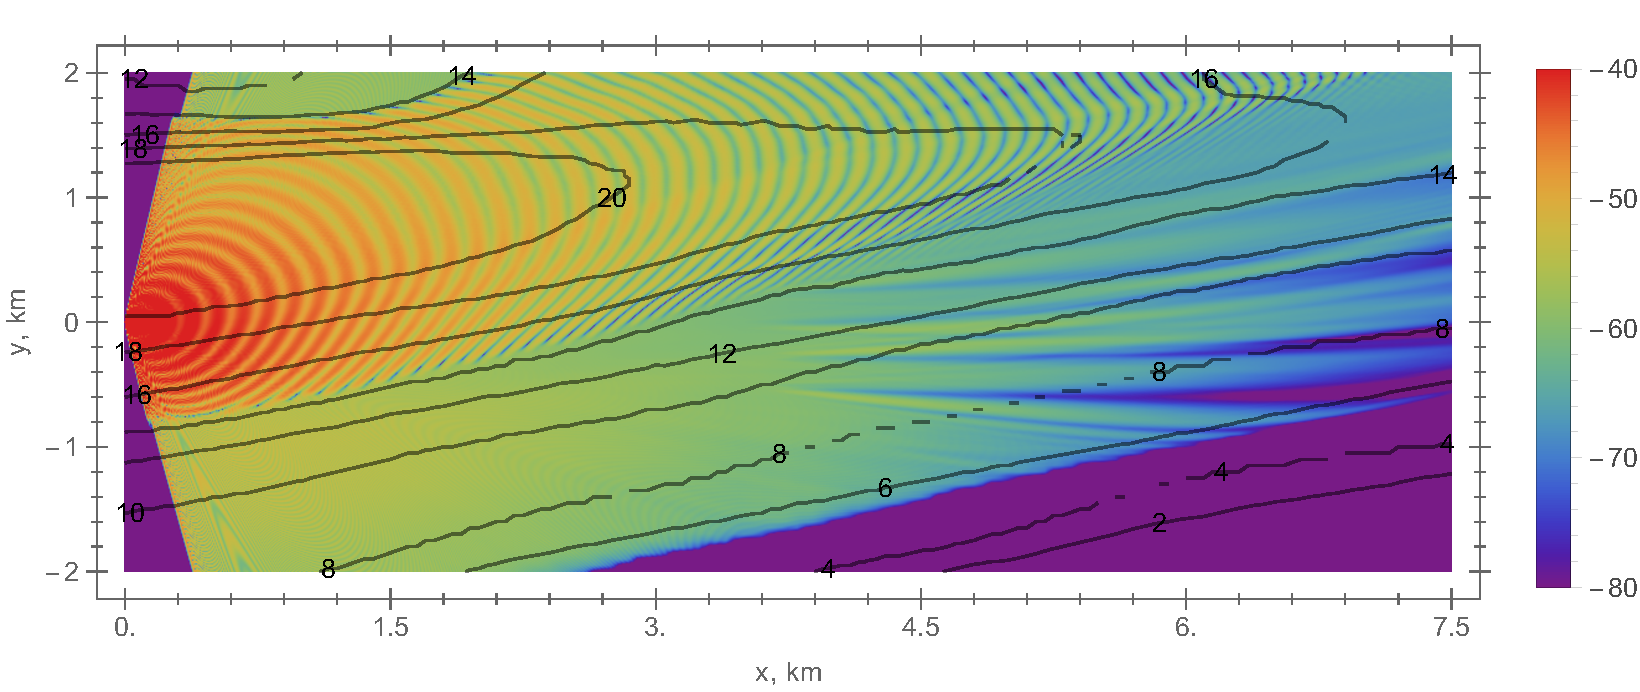
\includegraphics[width=\textwidth]{sakhalin_wampe_z4.pdf}
                        \caption{Решение \acrshort{wampe}, $z=4\ \text{м}$}
                    \end{subfigure}
                    \hfill
                    \begin{subfigure}[t]{0.75\textwidth}
                        \centering
                        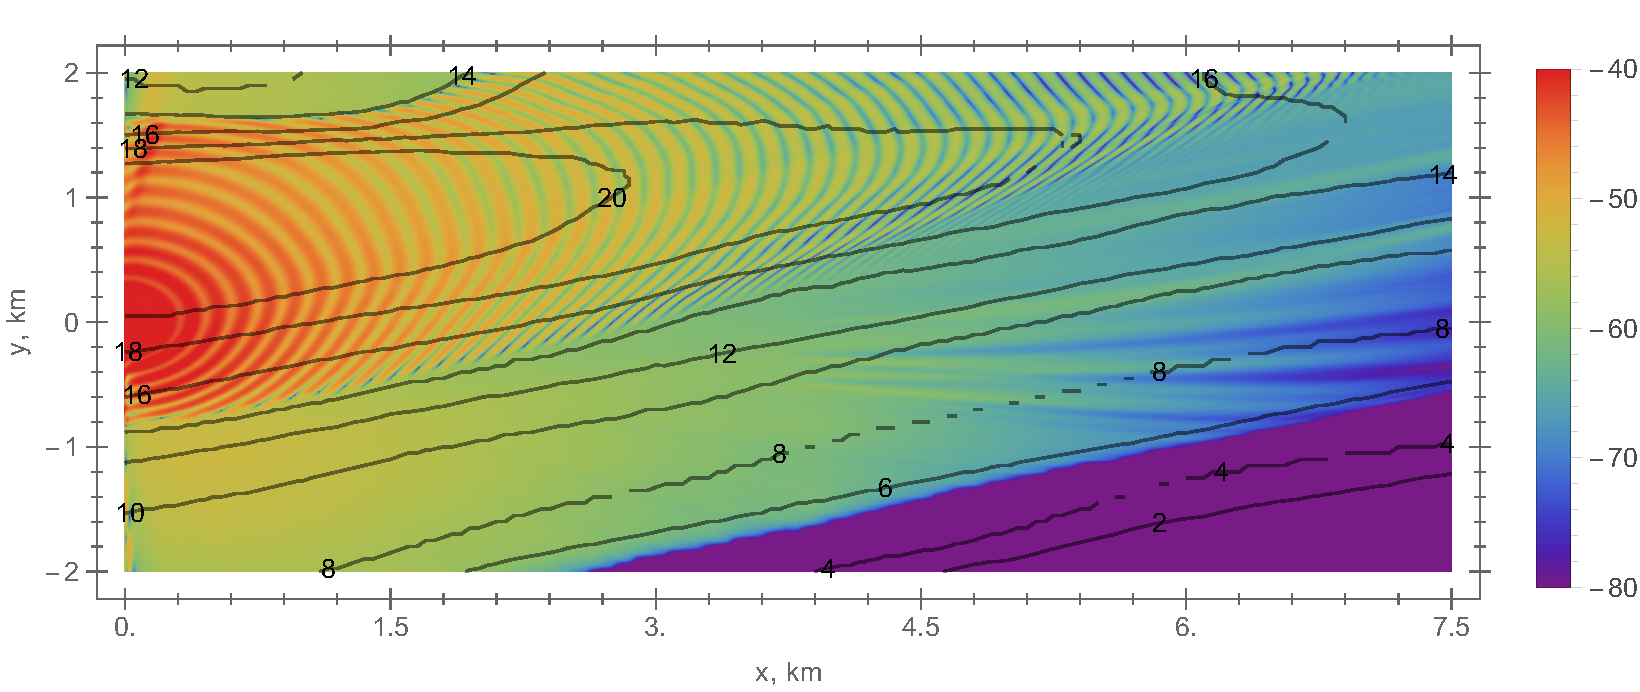
\includegraphics[width=\textwidth]{sakhalin_n11_z4.pdf}
                        \caption{\acrshort{ssp}, $z=4\ \text{м}$}
                    \end{subfigure}
                    \hfill
                    \begin{subfigure}[t]{0.75\textwidth}
                        \centering
                        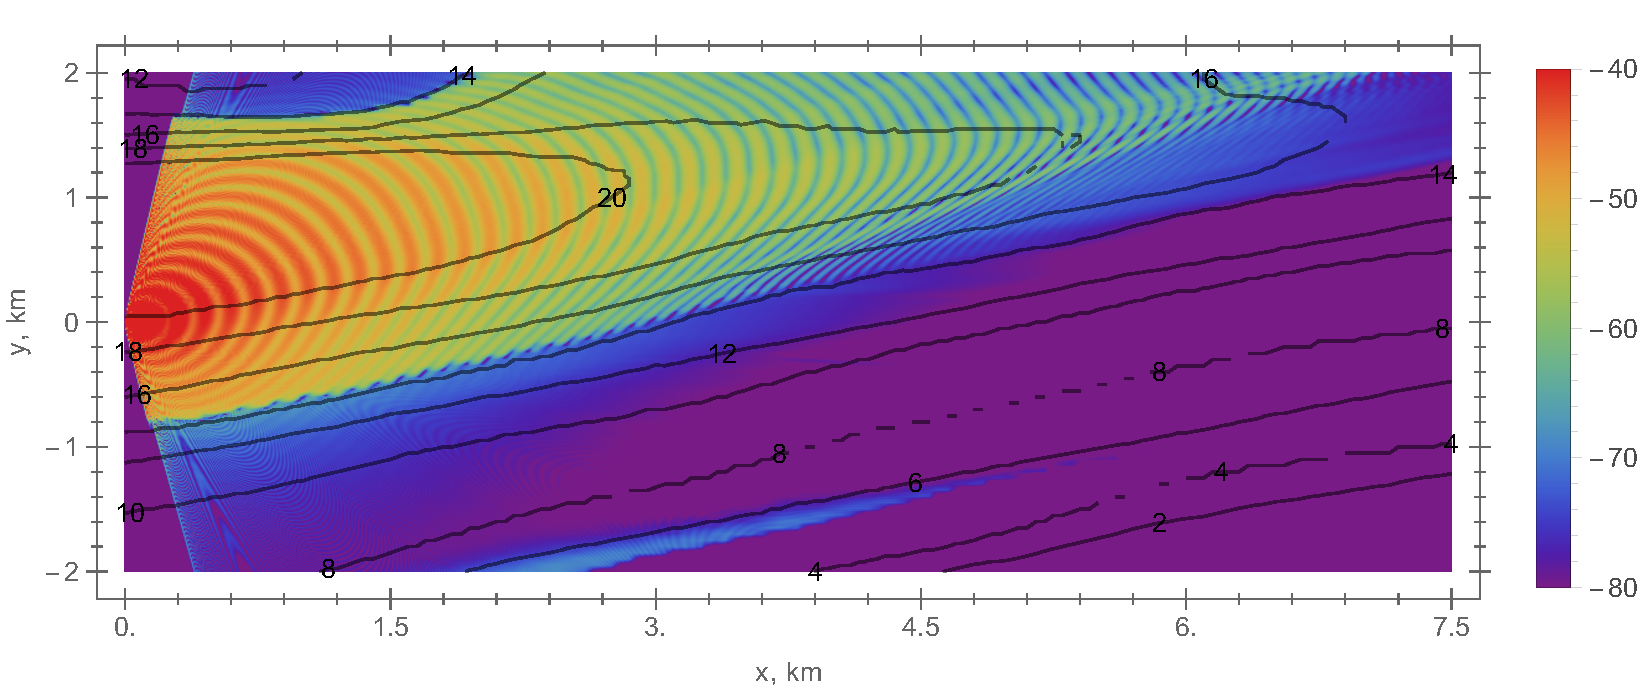
\includegraphics[width=\textwidth]{sakhalin_wampe_z20.pdf}
                        \caption{Решение \acrshort{wampe}, $z=20\ \text{м}$}
                    \end{subfigure}
                    \hfill
                    \begin{subfigure}[t]{0.75\textwidth}
                        \centering
                        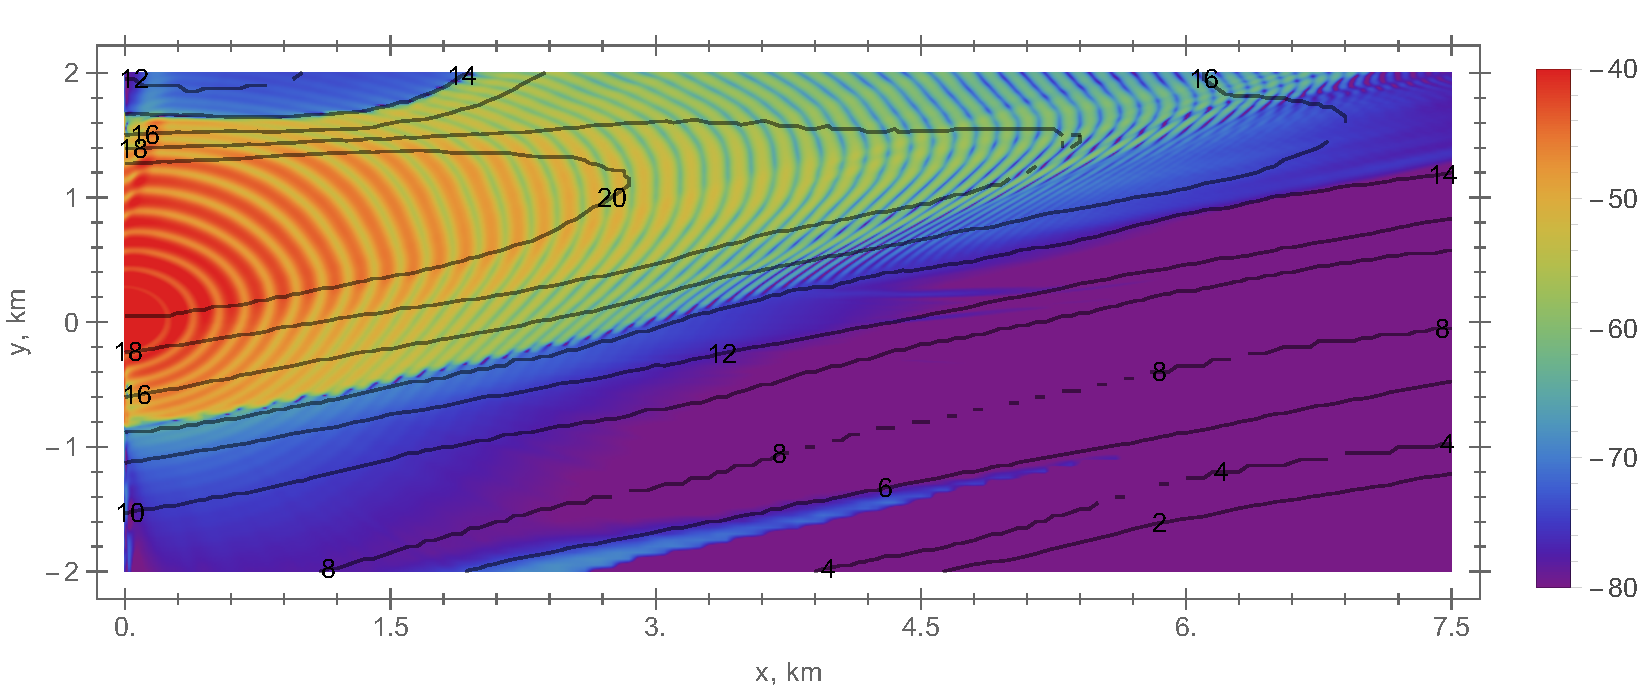
\includegraphics[width=\textwidth]{sakhalin_n11_z20.pdf}
                        \caption{\acrshort{ssp}, $z=20\ \text{м}$}
                    \end{subfigure}
                    \caption{Акустическое поле (в дБ отн. 1 м.) в волноводе с реальной батиметрией\label{fig::sakhalin_field}}
                \end{figure}
                \FloatBarrier
            \subsubsection{Результаты вычислительных экспериментов}
                \par В результате вычислительных экспериментов было показано, что разработанная численная схема с применением аппроксимации Паде произвольного порядка и лучевых начальных условий работает корректно и может быть использована в при моделировании распространения звука в сложных неоднородных океанических волноводах. При этом новый метод показывает значительно более гладкое и точное поле вблизи источника, а вдали от него учитывает волны исходящие под большими углами. Также в некоторых задачах более вычислительно затратные методы могут быть заменены разработанным методом, использование которого требует гораздо меньше вычислительных затрат.
\end{document}